\documentclass[10pt,a4paper]{article}
\usepackage[T1]{fontenc}
\usepackage[utf8]{inputenc}
\usepackage{lmodern}
\usepackage{newtxmath}
\usepackage[margin=20mm,top=18mm,bottom=17mm]{geometry}
\usepackage[table]{xcolor}
\usepackage{graphicx}
\usepackage{booktabs}
\usepackage{tabularx}
\usepackage{array}
\usepackage{ragged2e}
\usepackage{enumitem}
\usepackage{caption}
\usepackage{float}
\usepackage{microtype}
\usepackage{xurl}
\usepackage[hidelinks]{hyperref}
\usepackage{fancyhdr}
\hypersetup{
  pdftitle={MiniGrid Experiments for Continual Imagined Rehearsal},
  pdfauthor={Steven Davenport},
  pdfsubject={Task audition, sequential baseline, counterfactual-head pilot, and twin-Q qualification}
}
\definecolor{brandblue}{HTML}{2F6690}
\definecolor{rowgray}{HTML}{F5F7F9}
\definecolor{bodydark}{HTML}{222B35}
\definecolor{calloutblue}{HTML}{EAF2F8}
\definecolor{calloutgreen}{HTML}{EAF6EC}
\definecolor{calloutgreenborder}{HTML}{5A9A61}
\definecolor{calloutorange}{HTML}{FFF4E5}
\definecolor{calloutorangeborder}{HTML}{D89A45}
\color{bodydark}
\setlength{\parindent}{0pt}
\setlength{\parskip}{4.5pt plus 1pt}
\setlength{\emergencystretch}{2em}
\setcounter{secnumdepth}{0}
\setcounter{tocdepth}{2}
\renewcommand{\contentsname}{Contents}
\setlist{nosep,leftmargin=1.6em,topsep=3pt}
\captionsetup{font=small,justification=raggedright,singlelinecheck=false,skip=4pt}
\pagestyle{fancy}
\fancyhf{}
\fancyhead[L]{\scriptsize MiniGrid Continual Learning Experiments}
\fancyhead[R]{\scriptsize Continual Imagined Rehearsal}
\fancyfoot[C]{\scriptsize\thepage}
\renewcommand{\headrulewidth}{0.2pt}
\newcommand{\reportsection}[1]{\section{#1}}
\newcommand{\reportsubsection}[1]{\subsection{\textcolor{brandblue}{#1}}}
\begin{document}
\thispagestyle{plain}
\begin{center}
\vspace*{13mm}
{\LARGE\bfseries MiniGrid Experiments for\newline{}Continual Imagined Rehearsal\par}
\vspace{5mm}
{\large\color{brandblue} Task audition, visibility-first sequential baseline, counterfactual-head pilot, and twin-Q qualification:\newline{}acquisition, forgetting, goal semantics, and critic provenance\par}
\vspace{16mm}
{\normalsize Steven Davenport\par}
{\small Continual Reinforcement Learning Research Notes\par}
\vspace{7mm}
{\small Studies completed 30 August and 1 September 2026; report updated 2 September 2026\par}
\end{center}
\vspace{7mm}
\begin{center}\textbf{Abstract}\end{center}
\begingroup\small
This report records four MiniGrid studies in the Continual Imagined Rehearsal (CIR) programme. Study I trained six fixed-mission tasks independently for 100,000 environment steps over three seeds. It established that the reduced 12M DreamerV3 agent was neither uniformly saturated nor uniformly incapable, but rejected the assumption that the candidate tasks had equal difficulty: PutNear was reliable, GoToDoor, Fetch, and GoToObject were seed-sensitive, PickupDist was nearly unsolved, and UnlockPickup was never learned. That 1.8M-step audition completed in 5.14 hours.\par Study II then trained one goal-conditioned agent through GoToDoor, Fetch, GoToObject, and PutNear for 200,000 steps each. Three seeds were crossed with a 100k FIFO control, a uniform per-goal episode reservoir, and a reservoir sampled 50:50 between the current and all old goals. The 7.2M-step run evaluated all tasks every 50k and the active task every 25k under both sampled and deterministic policies, yielding 1,512 conditions and 75,600 episodes. Ninety read-only audits probed identical replay states at five phase boundaries. The complete workflow took 30.17 hours on one RTX 4090 with no failed scientific unit.\par Study II exposed a joint acquisition-retention failure. FIFO learned GoToDoor and PutNear but erased GoToDoor; 50:50 replay acquired three tasks but retained only 28.7\% GoToDoor success; uniform replay preserved teaching exposure but progressively starved the current task and ended at zero success on every task. Forward transfer was absent. Mechanistically, reward-event AUROC often approached one while same-state completion-goal top-1 accuracy remained weak. More seriously, the critic became grossly overoptimistic: uniform-reservoir value predictions reached 3.63 against a fixed realized-return mean of 0.077, the slow critic tracked the same error, and imagined targets were dominated by bootstrap value. Actor-selected imagination amplified the error.\par Study III then reran the matched seed-0 GoToDoor Phase-A case with one intervention: equal-weight oracle counterfactual supervision for reward and continuation on stop-gradient posterior features. Final success rose from 56\% to 88\% sampled and from 48\% to 86\% deterministic in this single seed. On completion states, factual reward was 0.844 while five wrong-goal rewards averaged 1.87e-6; factual stop probability was 0.99994 while wrong-goal stop probability averaged 0.00286. The unchanged critic remained flat at approximately 0.814-0.818 across all six goal queries, and wrong-goal imagined returns remained bootstrap-dominated. Counterfactual head training therefore causally repairs the measured reward/continuation semantics without making the critic a safe teacher. The pilot contains one task and one training seed and is not evidence about forgetting.\par Study IV froze the 400k two-goal representation and actor, then trained new discrete-action twin-Q critics from replay without the existing value head or a reward oracle. Across three Q initializations, counterfactual one-step relabelling reduced factual return MAE from 0.441 to 0.357, all-query Bellman MAE from 0.090 to 0.055, and twin disagreement from 0.056 to 0.043 relative to a dose-matched factual-only control. The same-state matching-minus-nonmatching value gap doubled from 0.157 to 0.322 and successful initial-state goal ranking rose from chance to 75.5\%. This qualifies ordinary counterfactual TD as a promising critic-training mechanism, but the offline two-goal study has no counterfactual return oracle and does not yet validate actor learning or CIR.
\endgroup
\clearpage
\tableofcontents
\clearpage
\reportsection{1. Research purpose and place in the programme}
The long-term goal is a safe continual reinforcement-learning agent that can adapt through imagined experience while minimizing unsafe or wasteful interaction with the real environment. Original Imagined Rehearsal was motivated by a basic problem in embodied reinforcement learning: a robot normally has to execute its current, possibly sub-optimal policy in the physical world to obtain feedback. Rehearsing within a learned world model offers a route to policy improvement before the next real action. Continual Imagined Rehearsal extends that premise across a changing task stream while explicitly addressing catastrophic forgetting, forward transfer, and adaptation safety [1].

RLScape remains central to that programme, but its 504-location click interface and long training cycles make it expensive to distinguish environment difficulty from agent failure. MiniGrid [2] provides a complementary diagnostic tier: it preserves partial visual observation, sparse goal completion, discrete control, randomized layouts, and multi-step behavior while reducing the action space to seven shared actions and shortening a full multi-seed matrix from days to hours.

This first MiniGrid study asks four questions:

\begin{enumerate}
\item Can a reduced DreamerV3 agent learn each candidate task within 100,000 environment steps without trivial early saturation?
\item Which tasks have comparable acquisition difficulty under an identical model, replay, and step budget?
\item Are conclusions sensitive to sampled versus deterministic action selection?
\item Which tasks are defensible candidates for the first continual sequence, and which should be deferred or redesigned?
\end{enumerate}
\begin{center}
\fcolorbox{brandblue}{calloutblue}{%
\begin{minipage}{0.94\linewidth}
\textbf{Claim boundary.} This is an independent-task difficulty audition. Each task and seed starts from a fresh agent. There are no task switches, no return to an earlier task, no imagined rehearsal intervention, and therefore no measurement of catastrophic forgetting, backward transfer, or forward transfer. The study selects the substrate on which those questions can later be tested.
\end{minipage}}
\end{center}
\reportsection{2. Study I: fixed-mission MiniGrid baseline}
\reportsubsection{2.1 Controlled task suite}
The stock task families were converted to fixed-mission variants so language parsing and episode-to-episode mission changes would not confound the first audition. Layouts, object positions, agent starts, and evaluation reset seeds still vary. All tasks expose the same seven-action MiniGrid interface: turn left, turn right, move forward, pick up, drop, toggle, and done. Observations are 64x64 partial RGB frames rendered from the agent's point of view.

\begin{table}[H]
\centering
\begingroup
\footnotesize
\setlength{\tabcolsep}{3.5pt}
\renewcommand{\arraystretch}{1.15}
\begin{tabularx}{\textwidth}{@{} >{\hsize=0.444\hsize\RaggedRight\arraybackslash}X >{\hsize=0.585\hsize\RaggedRight\arraybackslash}X >{\hsize=0.943\hsize\RaggedRight\arraybackslash}X >{\hsize=2.027\hsize\RaggedRight\arraybackslash}X @{}}
\rowcolor{brandblue}
\color{white}\textbf{Task} & \color{white}\textbf{Family} & \color{white}\textbf{Fixed mission} & \color{white}\textbf{Success and terminal behavior} \\
GoToDoor & navigation & go to the red door & Use done beside the unique red door; toggle or premature done terminates. \\
\rowcolor{rowgray}
Fetch & pickup & fetch the blue ball & Pick up the blue ball among two distractors; any pickup terminates. \\
GoToObject & navigation & go to the green key & Use done beside the green key; pickup, toggle, or premature done terminates. \\
\rowcolor{rowgray}
PutNear & pickup and place & put the yellow ball near the blue box & Carry and drop the ball in a neighboring cell; wrong pickup or any drop terminates. \\
UnlockPickup & unlock and pickup & pick up the only box behind the locked door & Find the key, unlock the door, enter the second room, and pick up the box. \\
\rowcolor{rowgray}
PickupDist & pickup & pick up the grey box & Pick up the grey box among four distractors; any pickup terminates. \\
\bottomrule
\end{tabularx}
\endgroup
\caption*{\textbf{Table 1.} Candidate tasks and their controlled success conditions.}
\end{table}
GoToDoor, Fetch, GoToObject, and PickupDist use 8x8 rooms; PutNear uses a 6x6 room; UnlockPickup uses the stock two-room geometry. Every episode is capped at 100 actions. Reward is sparse and positive only on success, with the standard MiniGrid time discount, so binary success is the primary comparison statistic and mean return also incorporates solution efficiency.

\reportsubsection{2.2 Agent and training configuration}
The agent is DreamerV3 [3] using the repository's reduced size12m preset. The observed optimizer namespace contained 10,499,273 parameters. The recurrent state-space model uses a deterministic state of width 2,048 and a 16x16 categorical stochastic state. Network width is 256. Training uses batches of eight sequences of length 32, imagination horizon 15, FIFO replay capacity 100,000, and a replay ratio of 32.

The visual dynamics remain goal-agnostic. A six-way one-hot goal\_id is concatenated into the reward, continuation, actor, and value heads. Although only one goal occurs within each independent run, this is the same interface intended for the later multi-task continual agent.

\begin{table}[H]
\centering
\begingroup
\footnotesize
\setlength{\tabcolsep}{3.5pt}
\renewcommand{\arraystretch}{1.15}
\begin{tabularx}{\textwidth}{@{} >{\hsize=0.639\hsize\RaggedRight\arraybackslash}X >{\hsize=1.357\hsize\RaggedRight\arraybackslash}X >{\hsize=0.608\hsize\RaggedRight\arraybackslash}X >{\hsize=1.396\hsize\RaggedRight\arraybackslash}X @{}}
\rowcolor{brandblue}
\color{white}\textbf{Component} & \color{white}\textbf{Setting} & \color{white}\textbf{Component} & \color{white}\textbf{Setting} \\
Observation & 64x64 partial RGB & Action space & Discrete(7) \\
\rowcolor{rowgray}
Model preset & size12m & Observed parameters & 10,499,273 \\
RSSM & deter 2048; hidden 256; classes 16 & Network width & 256 \\
\rowcolor{rowgray}
Batch & 8 sequences x 32 & Replay & FIFO, 100,000 \\
Train ratio & 32 & Environment instances & 1 \\
\rowcolor{rowgray}
Episode limit & 100 actions & Training budget & 100,000 steps/run \\
\bottomrule
\end{tabularx}
\endgroup
\caption*{\textbf{Table 2.} Pinned Dreamer and environment configuration.}
\end{table}
\reportsubsection{2.3 Experiment matrix and checkpoint evaluation}
The design is a fully crossed 6-task by 3-seed matrix. Each of the 18 agents trains for 100,000 environment steps with one environment instance and one training process active at a time. Immutable checkpoints are published at 25k, 50k, 75k, and 100k steps.

Each checkpoint is evaluated under both sampled and deterministic action selection. Every policy mode receives 50 episodes: 6 tasks x 3 seeds x 4 checkpoints x 2 modes x 50 episodes = \textbf{7,200 evaluation episodes}. The two policy modes for a task, seed, and checkpoint receive the same sequence of environment reset seeds. Adaptation is disabled, and namespace hashes verify that evaluation leaves the checkpoint unchanged.

\begin{figure}[H]
\centering
\begingroup
\footnotesize
\setlength{\tabcolsep}{3.5pt}
\renewcommand{\arraystretch}{1.15}
\begin{tabularx}{\textwidth}{@{} >{\hsize=0.741\hsize\RaggedRight\arraybackslash}X >{\hsize=0.975\hsize\RaggedRight\arraybackslash}X >{\hsize=1.014\hsize\RaggedRight\arraybackslash}X >{\hsize=1.271\hsize\RaggedRight\arraybackslash}X @{}}
\rowcolor{brandblue}
\color{white}\textbf{Fresh agent} & \color{white}\textbf{Training} & \color{white}\textbf{Milestones} & \color{white}\textbf{Paired evaluation} \\
task t, seed s & 100k steps; one env & 25k / 50k / 75k / 100k & 50 sampled + 50 deterministic \\
\bottomrule
\end{tabularx}
\endgroup
\caption*{\textbf{Figure 1.} Independent training and paired checkpoint evaluation protocol; repeated for six tasks and three seeds.}
\end{figure}
\reportsubsection{2.4 Predeclared difficulty rule}
Training difficulty uses binary episode success. For each episode, the analysis computes rolling success over the last $W=20$ episodes. Threshold time is the first environment step at which a full 20-episode window reaches 70\% success. Saturation time uses 90\%, and early saturation means reaching that level within the first 25,000 steps. Normalized training AUC integrates the rolling success curve over the 100k budget.

Two tasks are declared matched when both their mean normalized AUC and their median threshold step agree within a relative tolerance of 25\%. For two nonzero values a and b, max(|a|,|b|) / min(|a|,|b|) must be at most 1.25. The rule was fixed before results were analyzed. Its reliability limitation becomes important in Section 4.4.

\reportsubsection{2.5 Execution integrity and provenance}
The experiment is pinned to Git commit ae3cb917f661d6c3fe76422e476fc6179fbc694e, MiniGrid 3.1.0, Gymnasium 1.3.0, and JAX 0.4.33. The supervisor records the immutable specification digest, child commands, timing, return codes, timeouts, retries, and condition summaries. All 18 training attempts and all 144 evaluation attempts completed on their first attempt with return code zero. Every evaluation recorded exactly 50 episodes and 50 resets; all checkpoint hashes were equal before and after evaluation.

\clearpage
\reportsection{3. Operational result: a complete matrix in 5.14 hours}
The serial run started at 19:07:11 on 29 August 2026 and completed at 00:15:18 on 30 August 2026. Total wall time was 18,487.8 seconds, or 5.14 hours. Training children occupied 9,721.5 seconds and evaluation children 8,644.3 seconds, leaving roughly 122 seconds of orchestration overhead. Each 100k training run took about 540 seconds; each 50-episode evaluation condition took about 60 seconds.

\begin{table}[H]
\centering
\begingroup
\footnotesize
\setlength{\tabcolsep}{3.5pt}
\renewcommand{\arraystretch}{1.15}
\begin{tabularx}{\textwidth}{@{} >{\hsize=1.364\hsize\RaggedRight\arraybackslash}X >{\hsize=0.636\hsize\RaggedRight\arraybackslash}X >{\hsize=1.364\hsize\RaggedRight\arraybackslash}X >{\hsize=0.636\hsize\RaggedRight\arraybackslash}X @{}}
\rowcolor{brandblue}
\color{white}\textbf{Quantity} & \color{white}\textbf{Value} & \color{white}\textbf{Quantity} & \color{white}\textbf{Value} \\
Training units & 18 & Training steps & 1,800,000 \\
\rowcolor{rowgray}
Training episodes & 27,892 & Mean collection rate & 185.2 steps/s \\
Checkpoints & 72 & Evaluation conditions & 144 \\
\rowcolor{rowgray}
Evaluation episodes & 7,200 & Policy modes & 2 \\
Environment instances at once & 1 & Concurrent training units & 1 \\
\rowcolor{rowgray}
Retries or failed units & 0 & Final artifact footprint & 24 GB \\
Training child time & 2.70 h & Evaluation child time & 2.40 h \\
\rowcolor{rowgray}
Total wall time & 5.14 h & Orchestration overhead & 2.0 min \\
\bottomrule
\end{tabularx}
\endgroup
\caption*{\textbf{Table 3.} Experiment scale and operational outcome.}
\end{table}
\begin{center}
\fcolorbox{brandblue}{calloutblue}{%
\begin{minipage}{0.94\linewidth}
\textbf{Operational conclusion.} The speed came from the environment, not parallelism. The matrix used one environment, one training process, and serial task-seed units. MiniGrid therefore has further headroom for vectorized collection or concurrent seeds, but neither is required for fast baseline iteration.
\end{minipage}}
\end{center}
\reportsection{4. Learning results}
\reportsubsection{4.1 Checkpoint trajectories}
No task reached 90\% rolling training success in the first quarter of the budget, so the reduced agent was not trivially overpowered. The opposite problem occurred for UnlockPickup and PickupDist: the former never produced a success, while the latter remained close to zero.

\begin{figure}[H]
\centering
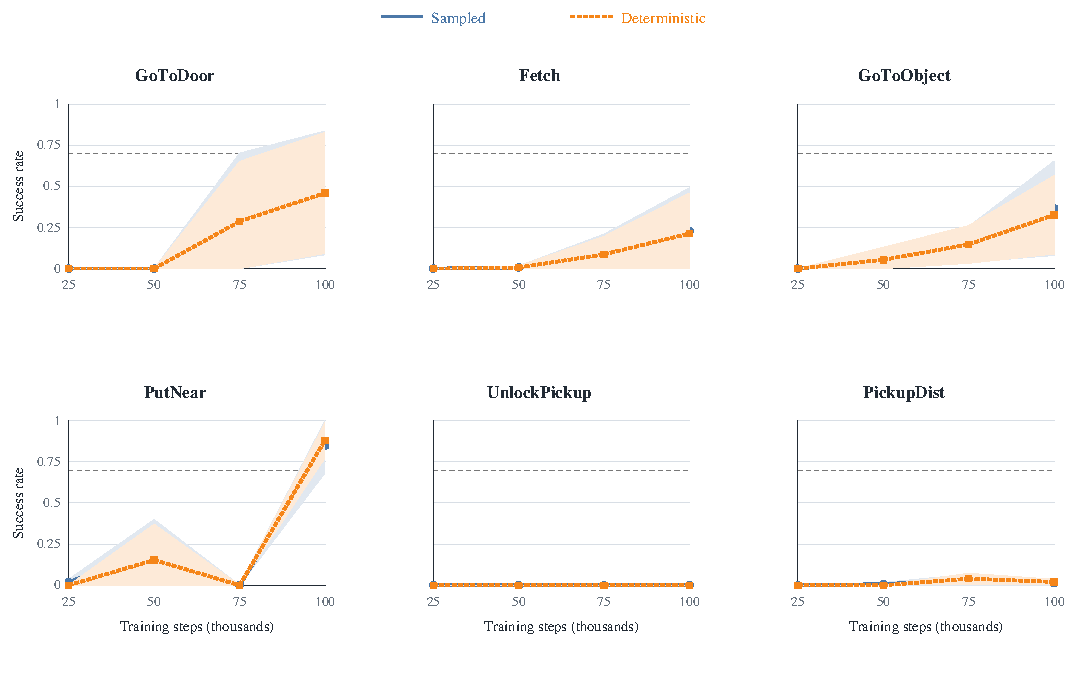
\includegraphics[width=\textwidth]{figures/figure_02.pdf}
\caption*{\textbf{Figure 2.} Checkpoint success by task and policy mode. Lines show the mean across three seeds; shaded regions show one population standard deviation. The dashed line marks 70\% success. Each point aggregates 150 evaluation episodes. PutNear's zero-success 75k checkpoint followed by strong 100k performance is a genuine non-monotonic result.}
\end{figure}
\begin{itemize}
\item \textbf{PutNear} was the only consistently strong task, ending at 84.7\% sampled and 88.0\% deterministic success. Its three seeds reached the rolling threshold, but the 75k checkpoint collapse shows instability.
\item \textbf{GoToDoor} learned late and inconsistently. It remained at zero through 50k, then reached 46.0\% final success under both policy modes.
\item \textbf{GoToObject} and \textbf{Fetch} showed gradual late learning but did not become reliable across seeds by 100k.
\item \textbf{UnlockPickup} produced zero training AUC and zero evaluation success at every checkpoint and seed.
\item \textbf{PickupDist} showed isolated successes but no sustained acquisition.
\end{itemize}
\reportsubsection{4.2 Final outcomes and seed heterogeneity}
\begin{table}[H]
\centering
\begingroup
\footnotesize
\setlength{\tabcolsep}{3.5pt}
\renewcommand{\arraystretch}{1.15}
\begin{tabularx}{\textwidth}{@{} >{\hsize=0.854\hsize\RaggedRight\arraybackslash}X >{\hsize=1.091\hsize\RaggedRight\arraybackslash}X >{\hsize=1.209\hsize\RaggedRight\arraybackslash}X >{\hsize=1.067\hsize\RaggedRight\arraybackslash}X >{\hsize=0.925\hsize\RaggedRight\arraybackslash}X >{\hsize=0.854\hsize\RaggedRight\arraybackslash}X @{}}
\rowcolor{brandblue}
\color{white}\textbf{Task} & \color{white}\textbf{Sampled success} & \color{white}\textbf{Deterministic success} & \color{white}\textbf{Training AUC} & \color{white}\textbf{Threshold seeds} & \color{white}\textbf{Median step} \\
GoToDoor & 46.0 +/- 37.6\% & 46.0 +/- 36.8\% & 0.154 +/- 0.139 & 2/3 & 82.4k \\
\rowcolor{rowgray}
Fetch & 22.7 +/- 26.4\% & 21.3 +/- 24.6\% & 0.059 +/- 0.026 & 1/3 & 98.0k \\
GoToObject & 36.7 +/- 28.7\% & 32.7 +/- 23.8\% & 0.066 +/- 0.043 & 0/3 & -- \\
\rowcolor{rowgray}
PutNear & 84.7 +/- 16.4\% & 88.0 +/- 10.7\% & 0.147 +/- 0.015 & 3/3 & 68.4k \\
UnlockPickup & 0.0 +/- 0.0\% & 0.0 +/- 0.0\% & 0.000 +/- 0.000 & 0/3 & -- \\
\rowcolor{rowgray}
PickupDist & 1.3 +/- 1.9\% & 2.0 +/- 1.6\% & 0.025 +/- 0.014 & 0/3 & -- \\
\bottomrule
\end{tabularx}
\endgroup
\caption*{\textbf{Table 4.} Final 100k-checkpoint outcomes. Mean +/- population SD over three seeds. Threshold seeds count runs reaching 70\% rolling training success.}
\end{table}
The means conceal strong between-seed structure. GoToDoor ranged from 0\% to 92\% sampled success; Fetch from 4\% to 60\%; and GoToObject from 0\% to 70\%. PutNear was the only task above 60\% in every seed and mode. This variance is central to experiment design: it determines whether later continual-learning differences can be distinguished from ordinary training luck.

\begin{figure}[H]
\centering
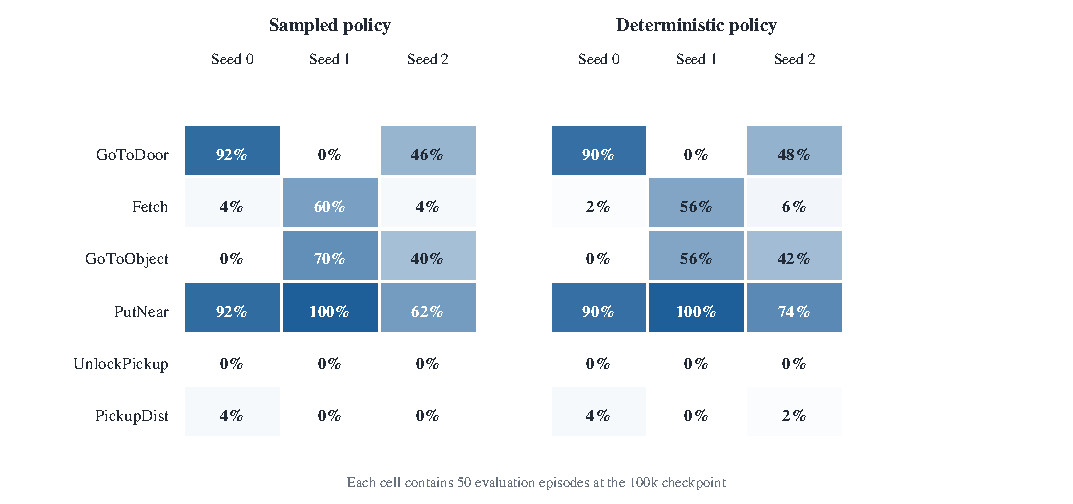
\includegraphics[width=\textwidth]{figures/figure_03.pdf}
\caption*{\textbf{Figure 3.} Final success for every task, seed, and policy mode. Each cell contains 50 episodes. The matrix exposes one successful Fetch seed, one failed GoToDoor seed, and the comparatively robust PutNear result.}
\end{figure}
\clearpage
\reportsubsection{4.3 Sampled and deterministic policies agree}
Across all 72 paired task-seed-checkpoint comparisons, sampled success exceeded deterministic success by only 0.42 percentage points on average. The mean absolute difference was 1.19 points, although the largest individual difference was 14 points. Most conditions lie on or near the identity line.

\begin{figure}[H]
\centering
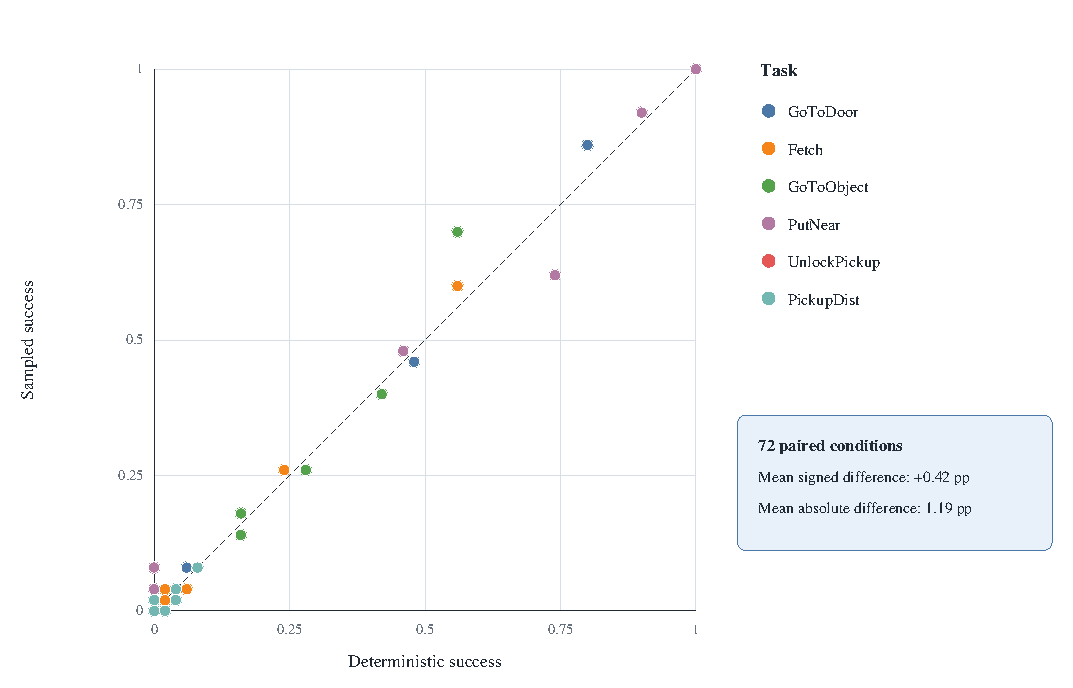
\includegraphics[width=\textwidth]{figures/figure_04.pdf}
\caption*{\textbf{Figure 4.} Agreement between sampled and deterministic success. Each point is one task, training seed, and checkpoint; paired modes use the same sequence of environment reset seeds.}
\end{figure}
Retaining both modes was useful confirmation rather than redundant bookkeeping. It verifies that the task ranking is not an artifact of one action convention. Small differences should not be over-interpreted with 50 episodes per condition. Both modes should remain in later CIR evaluations: deterministic behavior detects modal collapse, while sampled behavior represents the stochastic policy used by imagined rehearsal.

\reportsubsection{4.4 One formal pairwise match, but no qualified chain}
GoToDoor and PutNear have similar mean training AUC (0.154 versus 0.147), and their conditional median threshold times differ by less than 25\% (82.4k versus 68.4k). They are therefore the sole formal match among 15 task pairs. Neither the four-task alternating chain GoToDoor to Fetch to GoToObject to PutNear nor the progressive chain Fetch to PutNear to UnlockPickup passes all-pairs matching.

\begin{figure}[H]
\centering
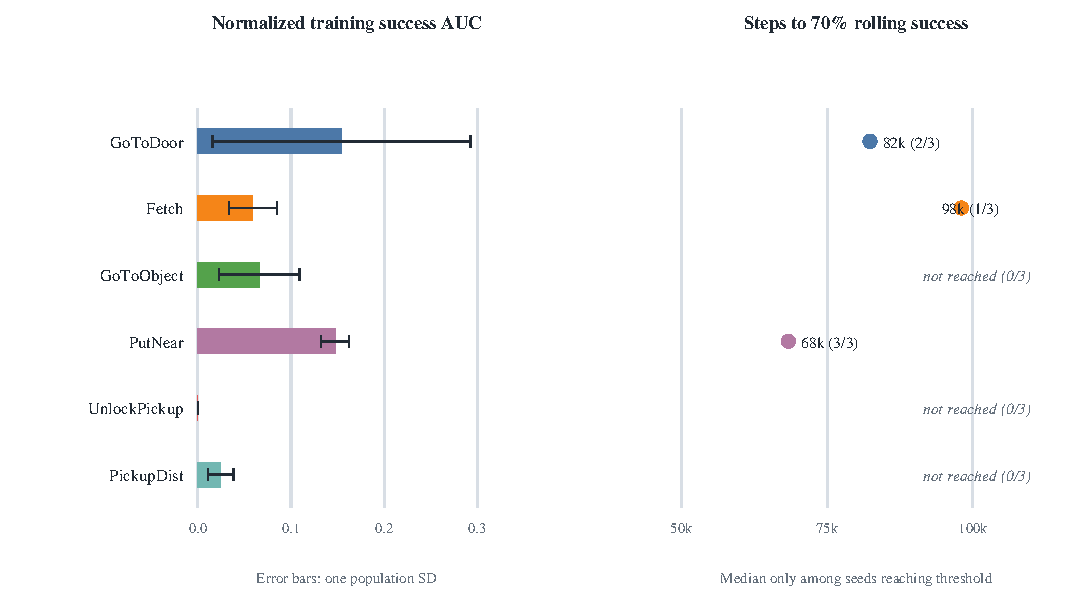
\includegraphics[width=\textwidth]{figures/figure_05.pdf}
\caption*{\textbf{Figure 5.} Predeclared task-difficulty statistics. AUC error bars show one population SD. Threshold labels report the median only among seeds reaching 70\%, followed by the number reaching it. This conditional definition allows GoToDoor and PutNear to pass despite different robustness.}
\end{figure}
\begin{table}[H]
\centering
\begingroup
\footnotesize
\setlength{\tabcolsep}{3.5pt}
\renewcommand{\arraystretch}{1.15}
\begin{tabularx}{\textwidth}{@{} >{\hsize=1.440\hsize\RaggedRight\arraybackslash}X >{\hsize=0.840\hsize\RaggedRight\arraybackslash}X >{\hsize=0.920\hsize\RaggedRight\arraybackslash}X >{\hsize=0.800\hsize\RaggedRight\arraybackslash}X @{}}
\rowcolor{brandblue}
\color{white}\textbf{Pair or chain} & \color{white}\textbf{AUC matched} & \color{white}\textbf{Threshold matched} & \color{white}\textbf{Overall} \\
GoToDoor - PutNear & yes & yes & matched \\
\rowcolor{rowgray}
GoToDoor - Fetch & no & yes & not matched \\
All other 13 pairs & mixed or no & no & not matched \\
\rowcolor{rowgray}
Alternating four-task chain & -- & -- & not qualified \\
Progressive three-task chain & -- & -- & not qualified \\
\bottomrule
\end{tabularx}
\endgroup
\caption*{\textbf{Table 5.} Pairwise and chain decision summary.}
\end{table}
\begin{center}
\fcolorbox{brandblue}{calloutblue}{%
\begin{minipage}{0.94\linewidth}
\textbf{Metric caveat.} Threshold time is calculated only among seeds that cross the threshold. PutNear crosses in 3/3 seeds; GoToDoor crosses in 2/3, and its AUC standard deviation is more than nine times PutNear's. The reproducible conclusion is one provisional match under the original rule, not two equally dependable tasks.
\end{minipage}}
\end{center}
\clearpage
\reportsection{5. Interpretation for continual imagined rehearsal}
\reportsubsection{5.1 Task-by-task interpretation}
\textbf{PutNear is the best present anchor.} It requires navigation, pickup, transport, and spatial placement, succeeds across all seeds, and does not saturate in the first quarter. Its 75k collapse nevertheless means checkpoint stability must be monitored; final performance alone would miss this behavior.

\textbf{GoToDoor is useful but underpowered as a sole navigation control.} Two seeds learn and one fails completely. This creates headroom for rehearsal but also a high false-positive risk: an apparent continual-learning effect could simply reflect initialization sensitivity.

\textbf{GoToObject and Fetch are promising intermediate candidates.} Both show genuine late acquisition in at least one seed and have neither a complete floor nor a reliable ceiling. More budget can reveal whether they converge. Their distinction also preserves task diversity: navigation-to-object versus target pickup among distractors.

\textbf{UnlockPickup is beyond the current learnability envelope.} A task that is never learned cannot measure forgetting. It may become valuable later as a forward-transfer or curriculum test after prerequisite behaviors are established.

\textbf{PickupDist is not interchangeable with Fetch.} Adding distractors reduces final success to approximately zero despite the identical action interface. It should be simplified, granted more training, or deferred.

\reportsubsection{5.2 The audition succeeds by rejecting a bad assumption}
The study did not find three or four equally difficult tasks, but this is not a failed experiment. It prevented the project from embedding a severe difficulty confound into the first CIR sequence. If UnlockPickup followed PutNear, later zero performance could be mislabelled catastrophic forgetting or unsafe rehearsal when the independent baseline already predicts zero. Conversely, combining PutNear and PickupDist would make aggregate retention dominated by unequal base learnability.

The speed advantage is decisive. RLScape remains necessary for validating the large discrete action interface and project-specific semantics, but MiniGrid can act as the mechanism-development tier. Complete independent baselines, ablations, and multi-seed safety checks can run before spending days on RLScape or moving toward simulated and physical robotic arms.

\reportsubsection{5.3 Recommended Stage II calibration}
No continual chain should be frozen from this study alone. The next calibration should retain the 12m agent and shared 100-action interface so task calibration is not confounded with a capacity change.

\begin{enumerate}
\item Extend GoToDoor, Fetch, GoToObject, and PutNear to 200k steps while retaining 25k checkpoints, testing whether weak tasks converge and whether PutNear remains stable.
\item Use at least five training seeds for the final candidate panel. Three seeds reveal instability but cannot characterize it precisely.
\item Replace the pairwise rule with a robustness-aware qualification: at least 4/5 seeds reach 70\%, no early saturation, final mean success in a target band such as 40-90\%, and acceptable between-seed dispersion.
\item Treat success, training AUC, threshold time, and checkpoint stability as separate axes instead of forcing one scalar ranking.
\item Defer UnlockPickup and PickupDist unless their mechanics are simplified or independent learning is demonstrated.
\end{enumerate}
For a short iteration before 200k runs, the current evidence supports a focused four-task audition panel: PutNear as reliable anchor, GoToDoor as variable navigation, GoToObject as intermediate navigation, and Fetch as intermediate pickup. This preserves navigation-pickup-navigation-placement diversity, but it is not yet an approved continual sequence.

\reportsubsection{5.4 Requirements for the first continual experiment}
Once tasks qualify independently, one shared goal-conditioned agent should train through a declared sequence and evaluate every encountered task at each phase boundary. The first continual study should include:

\begin{itemize}
\item a no-IR continual Dreamer baseline;
\item always-on reward-model-only imagined rehearsal as the primary positive comparator;
\item the same continual replay mechanism and real-environment step budget in every condition;
\item sampled and deterministic paired evaluations;
\item absolute success alongside average and maximum forgetting;
\item forward-transfer measurements against independent from-scratch learning curves;
\item a return phase that distinguishes retained competence from rapid reacquisition; and
\item hard integrity checks identifying which actor, critic, and world-model parameters may change during rehearsal.
\end{itemize}
\begin{center}
\fcolorbox{brandblue}{calloutblue}{%
\begin{minipage}{0.94\linewidth}
\textbf{Programme logic.} First establish that each component and task behaves as claimed. Then test whether rehearsal should run. Only after that should gating be judged as a safety and compute-control mechanism.
\end{minipage}}
\end{center}
\reportsection{6. Study II: visibility-first sequential baseline}
\reportsubsection{6.1 Objective and claim boundary}
Study II is the first true continual MiniGrid baseline. One shared goal-conditioned Dreamer trains through GoToDoor, Fetch, GoToObject, and PutNear, receiving 200,000 new environment steps per task. The sequence is navigation to pickup to navigation to pickup-and-place. It does not return to task A; the preserved 800k checkpoint permits that test later without changing this baseline.

The primary objective is visibility. In addition to acquisition, forgetting, backward transfer, and forward transfer, the run records replay composition, goal-specific training losses, actor drift on identical states, same-state reward and value calibration, and critic provenance under actor-selected versus recorded actions. This is deliberately a \textbf{no-IR baseline}: it contains no imagined rehearsal, counterfactual head training, critic regularization, or gate. Its role is to reveal what a future CIR intervention must repair and beat.

\begin{center}
\fcolorbox{brandblue}{calloutblue}{%
\begin{minipage}{0.94\linewidth}
\textbf{Interpretation boundary.} The replay arms are ordinary continual-learning controls, not CIR variants. A low forgetting score is not evidence of preservation when the corresponding task was never acquired. Counterfactual value queries are diagnostics, not supervised targets.
\end{minipage}}
\end{center}
\reportsubsection{6.2 Replay arms isolate memory from current-task exposure}
\begin{table}[H]
\centering
\begingroup
\footnotesize
\setlength{\tabcolsep}{3.5pt}
\renewcommand{\arraystretch}{1.15}
\begin{tabularx}{\textwidth}{@{} >{\hsize=0.710\hsize\RaggedRight\arraybackslash}X >{\hsize=0.788\hsize\RaggedRight\arraybackslash}X >{\hsize=1.068\hsize\RaggedRight\arraybackslash}X >{\hsize=1.435\hsize\RaggedRight\arraybackslash}X @{}}
\rowcolor{brandblue}
\color{white}\textbf{Arm} & \color{white}\textbf{Storage} & \color{white}\textbf{Sampling in phases A / B / C / D} & \color{white}\textbf{Question} \\
FIFO 100k & 100k transitions & current dominated after eviction & Forgetting control with short memory \\
\rowcolor{rowgray}
Uniform reservoir & about 1,000 episodes per goal & 100\% / 50\% / 33\% / 25\% current & Primary future-CIR baseline; preserve every old teaching signal \\
50:50 current/old & same per-goal reservoir & 100\% / 50\% / 50\% / 50\% current & Can ordinary current-biased replay solve the acquisition-retention trade-off? \\
\bottomrule
\end{tabularx}
\endgroup
\caption*{\textbf{Table 6.} Replay arms. The old half in the 50:50 arm is divided uniformly among represented old goals.}
\end{table}
All arms use the same 12M model, one environment, train ratio 32, 100-action limit, task order, seeds, and 7-action interface. Agent and optimizer snapshots are saved every 25k. Full replay is archived at each 200k phase boundary, making both exact resumption and later intervention studies possible.

\reportsubsection{6.3 Dense paired evaluation and read-only diagnostics}
The active task is evaluated every 25k; all four tasks are evaluated every 50k. Each condition uses 50 sampled and 50 deterministic episodes with paired reset seeds. The complete matrix is 3 arms x 3 seeds x 168 conditions per run = \textbf{1,512 evaluation conditions and 75,600 episodes}. Every evaluation verifies that the checkpoint parameter digest is unchanged.

After training, each seed's final uniform-reservoir replay fixes one state bank with up to 16 successful and 16 failed episodes per trained goal. Every arm's 0, 200k, 400k, 600k, and 800k snapshots is audited on the identical seed-specific bank. Forty-five head audits sweep all six goal queries over real posterior states; forty-five critic-provenance audits use 32 posterior samples, two anchors per episode, horizons 1, 3, 6, and 15, and both actor-selected and recorded-action proposals. All 90 audits preserve exact parameter hashes.

\reportsubsection{6.4 Operational result: 30.17 hours without a failed unit}
\begin{table}[H]
\centering
\begingroup
\footnotesize
\setlength{\tabcolsep}{3.5pt}
\renewcommand{\arraystretch}{1.15}
\begin{tabularx}{\textwidth}{@{} >{\hsize=1.287\hsize\RaggedRight\arraybackslash}X >{\hsize=0.690\hsize\RaggedRight\arraybackslash}X >{\hsize=1.333\hsize\RaggedRight\arraybackslash}X >{\hsize=0.690\hsize\RaggedRight\arraybackslash}X @{}}
\rowcolor{brandblue}
\color{white}\textbf{Quantity} & \color{white}\textbf{Value} & \color{white}\textbf{Quantity} & \color{white}\textbf{Value} \\
Training runs & 9 & Training phases & 36 \\
\rowcolor{rowgray}
Environment steps & 7,200,000 & Snapshots & 288 \\
Evaluation conditions & 1,512 & Evaluation episodes & 75,600 \\
\rowcolor{rowgray}
Head audits & 45 & Critic audits & 45 \\
Training child time & 10.53 h & Evaluation child time & 19.07 h \\
\rowcolor{rowgray}
Diagnostic child time & 0.51 h & Total wall time & 30.17 h \\
Recovered eval launches & 6 & Failed scientific units & 0 \\
\rowcolor{rowgray}
GPU concurrency & 1 process & Final artifact footprint & 80 GB \\
\bottomrule
\end{tabularx}
\endgroup
\caption*{\textbf{Table 7.} Sequential experiment scale and completion record. The run used one RTX 4090 from 31 August 00:06 to 1 September 06:16 BST.}
\end{table}
All 36 training phases completed in one attempt, with a mean of 17.54 minutes per 200k phase. Six evaluation processes received an immediate KeyboardInterrupt before scientific work and were automatically relaunched; their replacement conditions contain exactly 50 episodes and pass integrity validation. Diagnostics required no retry. The restart-safe supervisor reached its terminal marker and generated all aggregate tables.

\reportsection{7. Study II behavioral results}
\reportsubsection{7.1 Learning curves show both forgetting and acquisition interference}
\begin{figure}[H]
\centering
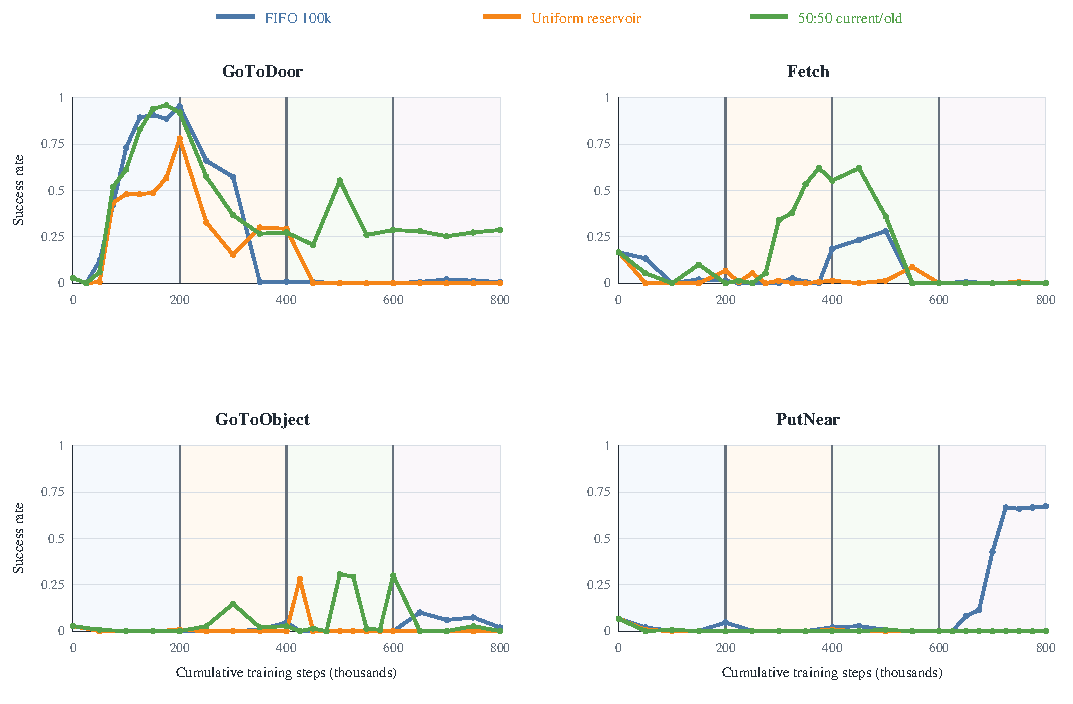
\includegraphics[width=\textwidth]{figures/figure_06.pdf}
\caption*{\textbf{Figure 6.} Sampled-policy success throughout the task stream. Each point is the mean over three seeds and 150 episodes. Vertical boundaries mark task switches at 200k, 400k, and 600k; colored backgrounds denote phases A-D. The FIFO arm learns the current task most readily but forgets old tasks. Reservoir replay reduces current-task exposure and often prevents acquisition before retention can be assessed.}
\end{figure}
\begin{itemize}
\item \textbf{GoToDoor is a clean forgetting case.} FIFO reaches 95.3\% immediately after phase A and finishes at 0.7\%. Uniform replay reaches 78.0\% and finishes at zero. The 50:50 arm reaches 92.0\% and retains 28.7\%.
\item \textbf{Fetch separates the replay arms.} FIFO acquires only 18.7\%; uniform replay only 1.3\%; the 50:50 arm reaches 55.3\%, then falls to zero by 800k.
\item \textbf{GoToObject remains difficult.} Only the 50:50 arm shows meaningful immediate acquisition, 30.0\%, and it too finishes at zero. Its weakness is not solely a forgetting effect.
\item \textbf{PutNear exposes current-task starvation.} FIFO, which is effectively current-only late in phase D, reaches and retains 67.3\%. Neither reservoir arm acquires it at all.
\end{itemize}
\reportsubsection{7.2 Acquisition and retention must be reported separately}
\begin{figure}[H]
\centering
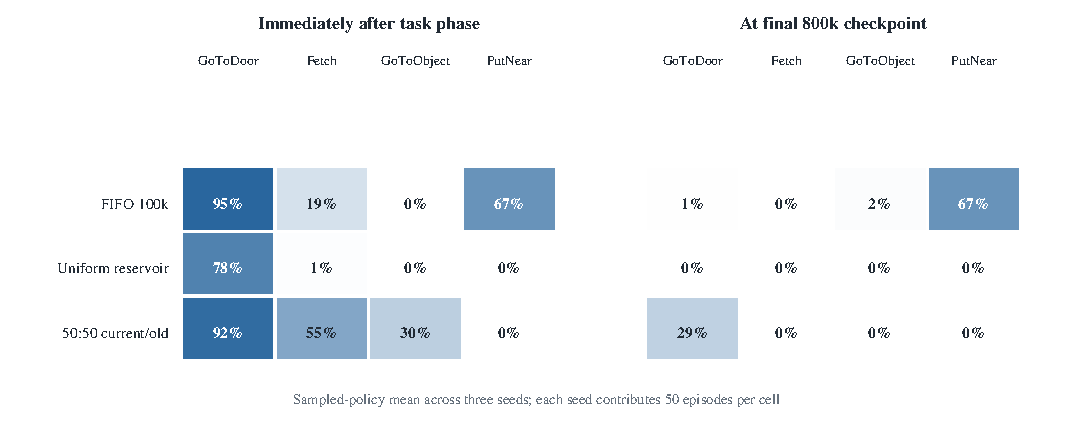
\includegraphics[width=\textwidth]{figures/figure_07.pdf}
\caption*{\textbf{Figure 7.} Immediate post-acquisition and final success. A low numerical forgetting score can arise because a task was never learned: uniform replay has lower mean forgetting than FIFO but ends with zero success everywhere.}
\end{figure}
\begin{table}[H]
\centering
\begingroup
\footnotesize
\setlength{\tabcolsep}{3.5pt}
\renewcommand{\arraystretch}{1.15}
\begin{tabularx}{\textwidth}{@{} >{\hsize=1.228\hsize\RaggedRight\arraybackslash}X >{\hsize=1.018\hsize\RaggedRight\arraybackslash}X >{\hsize=0.877\hsize\RaggedRight\arraybackslash}X >{\hsize=0.959\hsize\RaggedRight\arraybackslash}X >{\hsize=1.029\hsize\RaggedRight\arraybackslash}X >{\hsize=0.889\hsize\RaggedRight\arraybackslash}X @{}}
\rowcolor{brandblue}
\color{white}\textbf{Arm} & \color{white}\textbf{Post-acquisition} & \color{white}\textbf{Final success} & \color{white}\textbf{Peak forgetting} & \color{white}\textbf{Backward transfer} & \color{white}\textbf{Forward transfer} \\
FIFO 100k & 45.3\% & 17.5\% & 36.5\% & -27.8 pp & -5.0 pp \\
\rowcolor{rowgray}
Uniform reservoir & 19.8\% & 0.0\% & 22.0\% & -19.8 pp & -4.8 pp \\
50:50 current/old & 44.3\% & 7.2\% & 40.7\% & -37.2 pp & -5.8 pp \\
\bottomrule
\end{tabularx}
\endgroup
\caption*{\textbf{Table 8.} Sampled-policy means across four tasks and three seeds. Forgetting is peak post-acquisition minus final success; backward transfer is final minus immediate post-acquisition.}
\end{table}
There is no evidence of positive forward transfer. All three arms are slightly negative relative to each task's initial checkpoint, and pretraining success for later tasks is at or near zero. The main comparison is therefore not which arm transfers best, but where each arm lies on the acquisition-retention frontier. FIFO supplies the strongest phase-D acquisition; uniform replay supplies memory exposure but insufficient learning pressure; 50:50 recovers earlier acquisition without preventing later forgetting.

\reportsubsection{7.3 The realized replay mixtures match the intended intervention}
\begin{figure}[H]
\centering
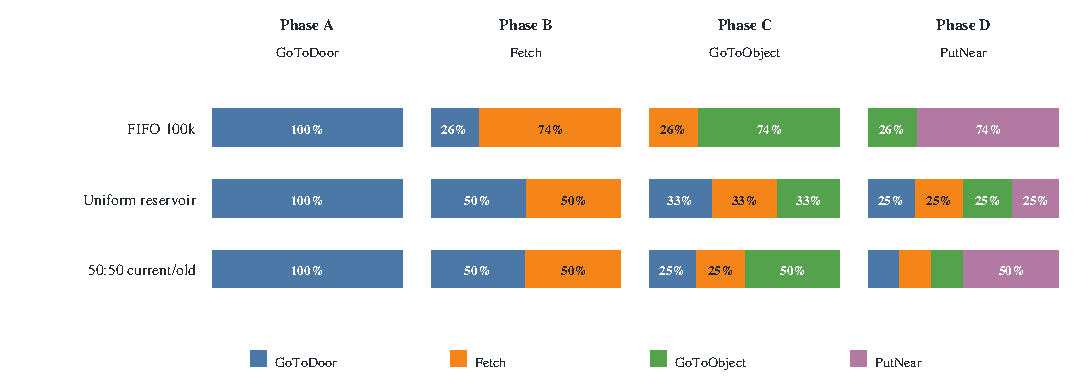
\includegraphics[width=\textwidth]{figures/figure_08.pdf}
\caption*{\textbf{Figure 8.} Observed training-batch goal fractions, averaged across seeds and within each phase. Uniform replay follows 100/50/33/25\% current exposure. The 50:50 arm holds the current task at 50\% after phase A. FIFO transitions gradually at each switch because its 100k capacity occupies half of a 200k phase.}
\end{figure}
The reservoir result is therefore not an implementation accident. Storage retained approximately 1,000 episodes per represented goal and the batch fractions match the declared policy. The failure is the scientific trade-off being tested: uniform preservation can make the current task only one quarter of phase-D updates. Even 50\% current exposure is insufficient for PutNear under multi-goal training, despite independent and FIFO evidence that the task is learnable.

\reportsubsection{7.4 Sampled and deterministic evaluations tell the same story}
The aggregate results remain stable under deterministic action selection. FIFO final success is 17.8\% rather than 17.5\%; uniform replay remains exactly zero; and 50:50 remains 7.2\%. Deterministic backward transfer differs from sampled by at most 2.2 percentage points at arm level. Maintaining both modes is still valuable: the agreement rules out action sampling as the source of collapse, while future IR may change policy entropy.

\reportsection{8. Study II component diagnostics}
\reportsubsection{8.1 Factual reward detection does not imply goal-conditioned teaching}
\begin{figure}[H]
\centering
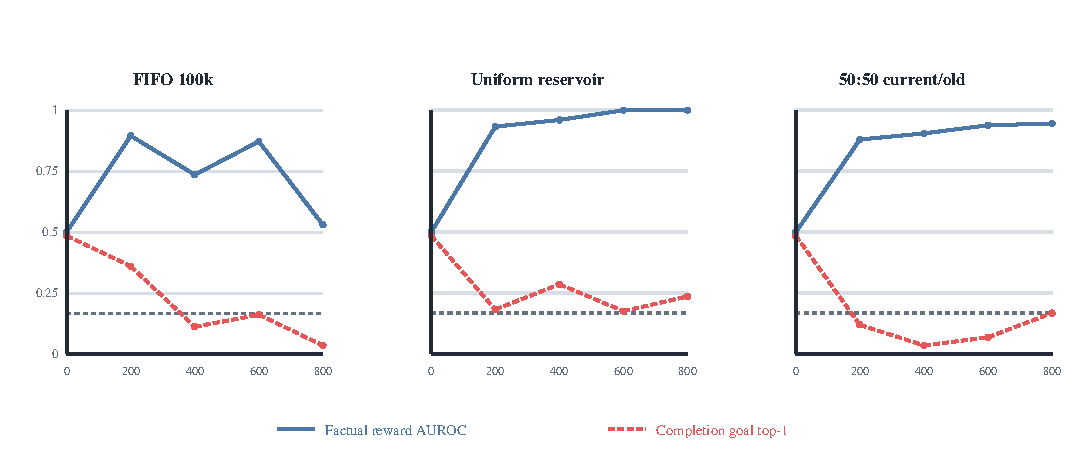
\includegraphics[width=\textwidth]{figures/figure_09.pdf}
\caption*{\textbf{Figure 9.} Reward-event recognition versus counterfactual goal selectivity on identical posterior states. Solid blue is factual reward AUROC; dashed red is top-1 identification of the completed goal when all six goal slots are queried. The horizontal dotted line is six-way chance. Means are over three seed-specific fixed state banks.}
\end{figure}
\begin{table}[H]
\centering
\begingroup
\scriptsize
\setlength{\tabcolsep}{3.5pt}
\renewcommand{\arraystretch}{1.15}
\begin{tabularx}{\textwidth}{@{} >{\hsize=1.389\hsize\RaggedRight\arraybackslash}X >{\hsize=0.953\hsize\RaggedRight\arraybackslash}X >{\hsize=1.045\hsize\RaggedRight\arraybackslash}X >{\hsize=0.820\hsize\RaggedRight\arraybackslash}X >{\hsize=0.873\hsize\RaggedRight\arraybackslash}X >{\hsize=1.032\hsize\RaggedRight\arraybackslash}X >{\hsize=0.887\hsize\RaggedRight\arraybackslash}X @{}}
\rowcolor{brandblue}
\color{white}\textbf{Arm at 800k} & \color{white}\textbf{Factual AUROC} & \color{white}\textbf{Average precision} & \color{white}\textbf{Goal top-1} & \color{white}\textbf{Reward margin} & \color{white}\textbf{Value prediction} & \color{white}\textbf{Value target} \\
FIFO 100k & 0.530 & 0.005 & 3.5\% & +0.000 & 0.714 & 0.077 \\
\rowcolor{rowgray}
Uniform reservoir & 1.000 & 0.996 & 23.6\% & +0.071 & 2.592 & 0.077 \\
50:50 current/old & 0.945 & 0.511 & 16.8\% & +0.031 & 1.132 & 0.077 \\
\bottomrule
\end{tabularx}
\endgroup
\caption*{\textbf{Table 9.} Final same-state head audit. Reward margin is matching minus nonmatching prediction at observed completion events; six-way top-1 chance is 16.7\%.}
\end{table}
This is the same conceptual failure seen in RLScape, now under a much cleaner action interface. The reservoir reward heads learn that a rare reward event occurred, but the requested goal changes that prediction only weakly. Uniform replay achieves nearly perfect factual classification while identifying the completed goal only 23.6\% of the time. The 50:50 top-1 rate is essentially chance. A factual reward head can therefore look excellent by AUROC and still be an unreliable counterfactual teacher for imagined rehearsal.

\reportsubsection{8.2 The critic becomes severely overoptimistic on real posterior states}
\begin{figure}[H]
\centering
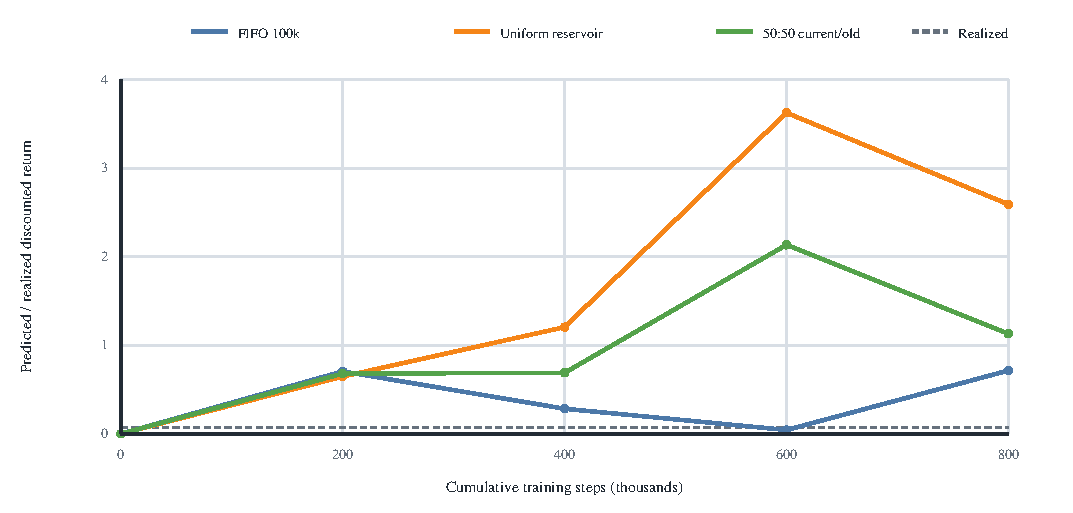
\includegraphics[width=\textwidth]{figures/figure_10.pdf}
\caption*{\textbf{Figure 10.} Online critic predictions on fixed real posterior states versus their realized inclusive discounted returns. Each line is a three-seed mean; the dashed realized target remains 0.077 because every arm and checkpoint is queried on the same seed-specific state bank. The critic error is present before imagination.}
\end{figure}
At 200k, critics already predict 0.65-0.71 against a realized mean of 0.077. The FIFO value later falls near the target at 600k but rebounds to 0.714 at 800k. Reservoir critics diverge much further: uniform replay reaches 3.626 at 600k, a +3.550 bias, while 50:50 reaches 2.134, a +2.058 bias. These values are structurally impossible as calibrated success returns in a task with at most one sparse reward.

The error is not a harmless intercept. At final checkpoints the value-return Pearson correlation is +0.110 for FIFO, -0.291 for uniform replay, and -0.133 for 50:50. Ranking is therefore weak or inverted. The slow critic does not provide an independent safeguard: its mean absolute difference from the online critic remains only 0.016, 0.026, and 0.010 respectively at 800k, tiny relative to the calibration error.

\reportsubsection{8.3 Standard imagined returns inherit and amplify the critic error}
\begin{figure}[H]
\centering
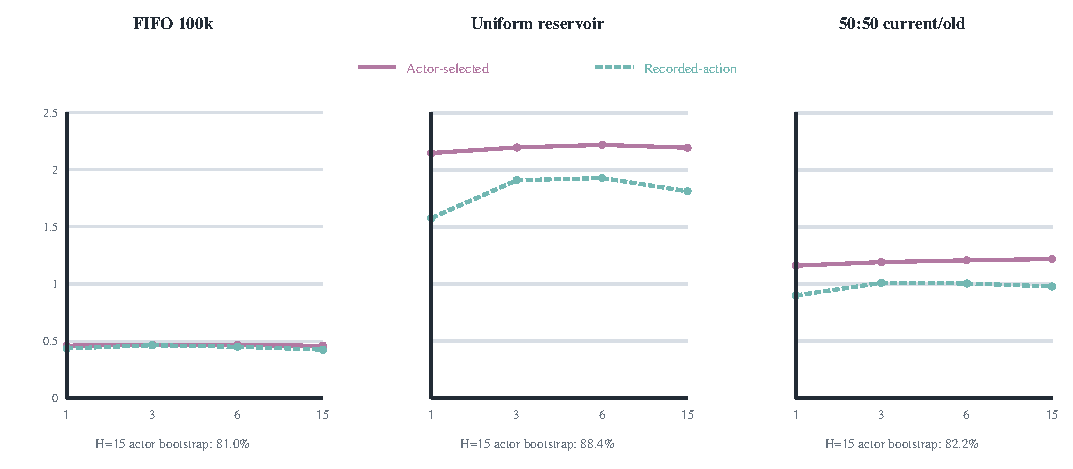
\includegraphics[width=\textwidth]{figures/figure_11.pdf}
\caption*{\textbf{Figure 11.} Factual imagined return under actor-selected and recorded-action proposals, pooled across trained checkpoints and three seeds. Every point uses the same posterior anchors. Actor selection amplifies predicted return most strongly in the reservoir arms; annotations report the actor target's bootstrap fraction at H=15.}
\end{figure}
\begin{table}[H]
\centering
\begingroup
\footnotesize
\setlength{\tabcolsep}{3.5pt}
\renewcommand{\arraystretch}{1.15}
\begin{tabularx}{\textwidth}{@{} >{\hsize=1.269\hsize\RaggedRight\arraybackslash}X >{\hsize=0.831\hsize\RaggedRight\arraybackslash}X >{\hsize=0.923\hsize\RaggedRight\arraybackslash}X >{\hsize=1.073\hsize\RaggedRight\arraybackslash}X >{\hsize=0.958\hsize\RaggedRight\arraybackslash}X >{\hsize=0.946\hsize\RaggedRight\arraybackslash}X @{}}
\rowcolor{brandblue}
\color{white}\textbf{Arm} & \color{white}\textbf{Actor H15} & \color{white}\textbf{Recorded H15} & \color{white}\textbf{Actor amplification} & \color{white}\textbf{Reward-only H15} & \color{white}\textbf{Bootstrap fraction} \\
FIFO 100k & 0.459 & 0.425 & +0.034 & 0.154 & 81.0\% \\
\rowcolor{rowgray}
Uniform reservoir & 2.194 & 1.812 & +0.381 & 0.103 & 88.4\% \\
50:50 current/old & 1.219 & 0.978 & +0.240 & 0.148 & 82.2\% \\
\bottomrule
\end{tabularx}
\endgroup
\caption*{\textbf{Table 10.} Pooled factual H=15 imagined-target decomposition over 200k-800k checkpoints. Full target equals predicted reward contribution plus critic bootstrap under Dreamer's continuation-weighted return.}
\end{table}
Recorded actions already produce overoptimistic targets, so policy exploitation is not the origin of the error. Actor-selected actions then raise the target by 0.381 in uniform replay and 0.240 in 50:50 replay. Predicted reward remains small relative to the full target; the critic bootstrap contributes 81-88\% even at H=15 and approximately 97-99\% at H=1. Standard critic-bootstrapped IR would consequently train the actor toward a signal known to be miscalibrated on both real and imagined states.

\reportsubsection{8.4 Actor drift confirms that preserved components do not preserve behavior}
The same-state actor audit compares factual-goal action distributions at adjacent phase boundaries. Mean Jensen-Shannon divergence per switch is 0.371 for FIFO, 0.373 for uniform replay, and 0.306 for 50:50. Modal action agreement is only 27.3\%, 35.0\%, and 47.6\% respectively. The 50:50 actor changes less, but its retained behavior is still poor. These data reinforce a crucial distinction: replay can keep old examples and stabilize parameters without retaining a competent goal-conditioned policy.

\reportsection{9. Study III: counterfactual-head Phase-A pilot}
\reportsubsection{9.1 Question and single-factor intervention}
Study II showed that factual reward detection can coexist with weak goal semantics, but its read-only audit was correlational. Study III makes the causal intervention: rerun only the seed-0 uniform-reservoir GoToDoor phase from scratch while changing reward and continuation supervision. The question is whether explicit negative labels for the five nonmatching goal queries repair same-state semantics without preventing factual task acquisition.

\begin{table}[H]
\centering
\begingroup
\footnotesize
\setlength{\tabcolsep}{3.5pt}
\renewcommand{\arraystretch}{1.15}
\begin{tabularx}{\textwidth}{@{} >{\hsize=0.725\hsize\RaggedRight\arraybackslash}X >{\hsize=1.099\hsize\RaggedRight\arraybackslash}X >{\hsize=1.175\hsize\RaggedRight\arraybackslash}X @{}}
\rowcolor{brandblue}
\color{white}\textbf{Component} & \color{white}\textbf{Matched standard Phase A} & \color{white}\textbf{Counterfactual-head pilot} \\
Task / seed / budget & GoToDoor / 0 / 200k & GoToDoor / 0 / 200k \\
\rowcolor{rowgray}
Agent / replay & 12M Dreamer; uniform reservoir & identical \\
Factual reward and continuation & ordinary observed targets & unchanged \\
\rowcolor{rowgray}
Five wrong-goal queries & no explicit target & reward = 0; factual completion continues \\
Physical terminal & stops the factual goal & stops every goal \\
\rowcolor{rowgray}
Counterfactual feature path & not present & stop-gradient posterior features \\
Actor / critic objectives & ordinary Dreamer & unchanged; no regularization \\
\rowcolor{rowgray}
Evaluation & 9 checkpoints x 2 modes x 50 episodes & same reset and policy-RNG schedule \\
\bottomrule
\end{tabularx}
\endgroup
\caption*{\textbf{Table 11.} Matched Phase-A intervention contract. The counterfactual loss is averaged over the five nonmatching goals and has equal weight to the factual head loss.}
\end{table}
The added path receives stopped posterior features, so it can update only the reward and continuation heads. It cannot alter the encoder or RSSM through the counterfactual loss. The actor, online critic, slow critic, their targets, and their objectives remain untouched. This isolates head semantics from generic critic regularization and from the CIR behavior-learning mechanism itself.

\reportsubsection{9.2 Execution integrity and factual acquisition}
The run completed 200,000/200,000 environment steps, all 18 checkpoint-policy evaluation conditions, and all four read-only diagnostic jobs with no failed scientific attempt. Nine immutable snapshots cover 0-200k at 25k intervals. Every evaluation contains exactly 50 episodes and 50 resets with unchanged checkpoint hashes; the 0k and 200k head and critic audits also preserve parameter hashes. The supervisor reached terminal status \emph{complete} 39.35 minutes after its recorded creation time on the RTX 4090.

\begin{figure}[H]
\centering
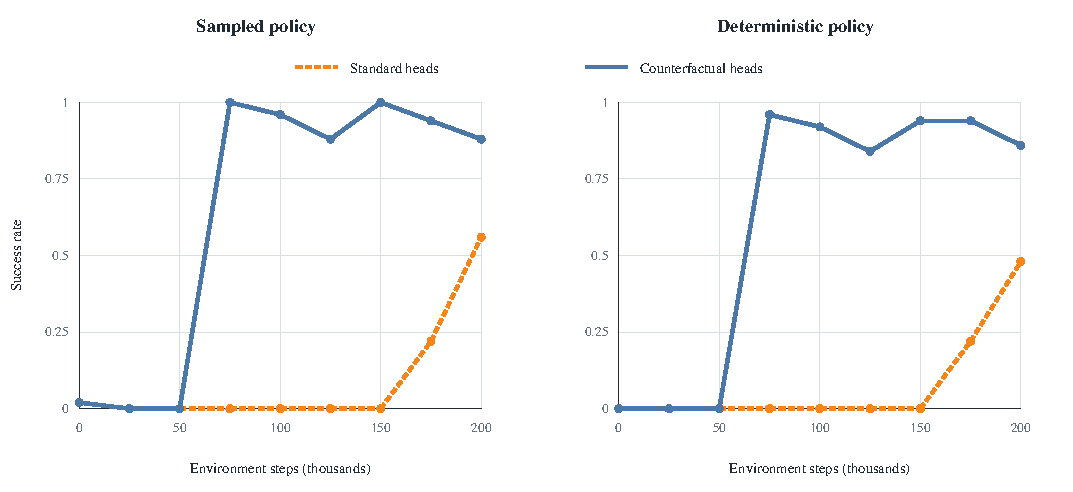
\includegraphics[width=\textwidth]{figures/figure_12.pdf}
\caption*{\textbf{Figure 12.} GoToDoor success for the matched standard-training and counterfactual-head seed-0 Phase-A runs. Each point is 50 episodes; sampled and deterministic modes use the same reset identities and paired policy random-key schedule in both runs. This is one training seed, so the earlier acquisition and final gap are descriptive, not a population-level performance claim.}
\end{figure}
\begin{table}[H]
\centering
\begingroup
\footnotesize
\setlength{\tabcolsep}{3.5pt}
\renewcommand{\arraystretch}{1.15}
\begin{tabularx}{\textwidth}{@{} >{\hsize=1.102\hsize\RaggedRight\arraybackslash}X >{\hsize=0.982\hsize\RaggedRight\arraybackslash}X >{\hsize=0.922\hsize\RaggedRight\arraybackslash}X >{\hsize=1.018\hsize\RaggedRight\arraybackslash}X >{\hsize=0.922\hsize\RaggedRight\arraybackslash}X >{\hsize=1.054\hsize\RaggedRight\arraybackslash}X @{}}
\rowcolor{brandblue}
\color{white}\textbf{Policy mode} & \color{white}\textbf{Initial standard} & \color{white}\textbf{Initial pilot} & \color{white}\textbf{Final standard} & \color{white}\textbf{Final pilot} & \color{white}\textbf{Final difference} \\
Sampled & 2\% & 2\% & 56\% & 88\% & +32 pp \\
\rowcolor{rowgray}
Deterministic & 0\% & 0\% & 48\% & 86\% & +38 pp \\
\bottomrule
\end{tabularx}
\endgroup
\caption*{\textbf{Table 12.} Matched seed-0 GoToDoor evaluation at 0 and 200k. Every cell contains 50 episodes; sampled and deterministic results are not pooled.}
\end{table}
Factual learning was therefore not degraded in the prespecified case. The pilot first reached high checkpoint success at 75k and remained between 84\% and 100\% through 200k, whereas the matched standard run remained at zero through 150k before reaching 56\% sampled and 48\% deterministic success. This is compatible with a useful acquisition effect, but one seed cannot distinguish a robust benefit from training-path sensitivity.

\reportsubsection{9.3 Counterfactual supervision repairs reward and continuation semantics}
\begin{figure}[H]
\centering
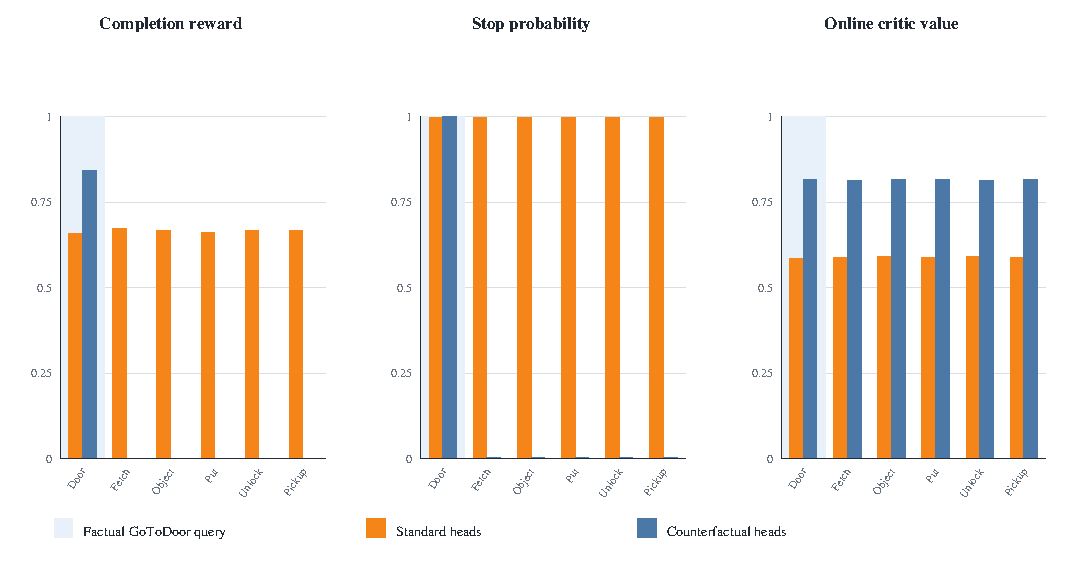
\includegraphics[width=\textwidth]{figures/figure_13.pdf}
\caption*{\textbf{Figure 13.} Six-goal queries on GoToDoor completion states at 200k. Within each run, the posterior state is held fixed and only the queried goal changes; each bar summarizes 16 completion events. The standard and pilot diagnostics use their own immutable final-replay state banks, so cross-run heights are descriptive while each within-run goal contrast is exact. Stop probability is one minus predicted continuation.}
\end{figure}
The repair is nearly complete on the measured completion semantics. Factual reward reaches 0.844063 with AUROC and average precision both 1.0. The five nonmatching completion rewards lie between 1.78e-6 and 1.92e-6, giving a factual-minus-nonmatching margin of 0.844061 and six-way completion-goal top-1 accuracy of 100\%. The standard reference instead assigns 0.659 factual reward and 0.661-0.672 to wrong goals on its GoToDoor completion bank.

Continuation changes in the intended direction as well. Under the factual query, completion continuation is 0.0000585, or stop probability 0.9999415. Under the five wrong-goal queries, continuation is 0.997119-0.997157, or stop probability only 0.002843-0.002882. Standard training predicts a stop probability above 0.999 for both factual and wrong goals. Counterfactual supervision has therefore taught the heads that the same physical event completes GoToDoor but does not terminate the other task objectives.

\reportsubsection{9.4 The unchanged critic does not inherit goal selectivity}
The clean head repair does not propagate automatically into the critic. On the same pilot completion states, the online critic predicts 0.817672 for GoToDoor and 0.813715-0.817463 for the five wrong goals; the complete six-query range is only 0.003957. The slow critic is similarly flat at 0.815326-0.819497. Across all 972 audited GoToDoor states, the online critic predicts a mean inclusive return of 0.750510 against a realized mean of 0.182932, a +0.567578 bias. Correct reward semantics are therefore not sufficient to calibrate or goal-separate the unchanged Dreamer value objective in this run.

\begin{table}[H]
\centering
\begingroup
\scriptsize
\setlength{\tabcolsep}{3.5pt}
\renewcommand{\arraystretch}{1.15}
\begin{tabularx}{\textwidth}{@{} >{\hsize=0.409\hsize\RaggedRight\arraybackslash}X >{\hsize=1.037\hsize\RaggedRight\arraybackslash}X >{\hsize=1.105\hsize\RaggedRight\arraybackslash}X >{\hsize=1.146\hsize\RaggedRight\arraybackslash}X >{\hsize=1.133\hsize\RaggedRight\arraybackslash}X >{\hsize=1.160\hsize\RaggedRight\arraybackslash}X >{\hsize=1.010\hsize\RaggedRight\arraybackslash}X @{}}
\rowcolor{brandblue}
\color{white}\textbf{H} & \color{white}\textbf{Factual full} & \color{white}\textbf{Factual reward} & \color{white}\textbf{Factual bootstrap} & \color{white}\textbf{Wrong-goal full} & \color{white}\textbf{Wrong-goal reward} & \color{white}\textbf{Wrong bootstrap} \\
1 & 0.812 & 0.187 & 78.7\% & 0.796 & 5.29e-07 & 100.00\% \\
\rowcolor{rowgray}
3 & 0.825 & 0.233 & 73.6\% & 0.788 & 0.0002 & 99.98\% \\
6 & 0.827 & 0.354 & 59.3\% & 0.688 & 0.0009 & 99.68\% \\
\rowcolor{rowgray}
15 & 0.827 & 0.515 & 39.3\% & 0.516 & 0.0033 & 98.96\% \\
\bottomrule
\end{tabularx}
\endgroup
\caption*{\textbf{Table 13.} Actor-selected imagined-return decomposition at the pilot 200k checkpoint. Full return equals predicted reward contribution plus critic bootstrap under the continuation-weighted target; wrong-goal rows pool the five nonmatching queries.}
\end{table}
The imagination audit makes the residual failure operational. At H=15 the corrected wrong-goal reward-only contribution is 0.0033, yet the full wrong-goal return is 0.516 because 98.96\% of its magnitude is attributed to critic bootstrap. At H=1 the wrong-goal reward contribution is effectively zero while the full target remains 0.796. An actor trained with the standard bootstrapped IR objective would still receive a large positive signal for goals that the reward and continuation heads now correctly reject.

\reportsubsection{9.5 Interpretation and claim boundary}
\begin{center}
\fcolorbox{brandblue}{calloutblue}{%
\begin{minipage}{0.94\linewidth}
\textbf{Causal result.} Explicit counterfactual labels repair the measured reward and continuation goal semantics while preserving factual GoToDoor learning. Because the critic objective was unchanged, its flat cross-goal values isolate the next unresolved mechanism rather than weakening the head result.
\end{minipage}}
\end{center}
This pilot does not show that counterfactual heads reduce catastrophic forgetting, generalize across tasks or training seeds, or make critic-bootstrapped rehearsal safe. It also supplies no oracle counterfactual actor or critic target. Extending the same labels mechanically into those objectives would overlap with the CIR method and requires a separately derived target and controls against bootstrap leakage.

\clearpage
\reportsection{10. Study IV: offline counterfactual twin-Q qualification}
\reportsubsection{10.1 Question and controlled critic target}
Study III rejects the proposed upstream-propagation explanation: explicitly fixing reward and continuation conditioning did not make the unchanged Dreamer critic selective or calibrated. Study IV asks the next narrow question: can an ordinary counterfactual one-step temporal-difference objective train a goal-selective critic without an oracle value, the existing optimistic critic, or a 15-step imagined return?

The source is the seed-0 50:50-current/old checkpoint immediately after Fetch at 400k. Its frozen policy solved Fetch at 84\% sampled and 90\% deterministic success but scored zero on GoToDoor in both modes, supplying an intentionally asymmetric acquired/forgotten two-goal state distribution. The encoder, RSSM, actor, reward and continuation heads, and both original value heads are frozen. New near-zero discrete-action twin-Q networks receive posterior features and a GoToDoor or Fetch query and emit values for all seven actions.

\begin{table}[H]
\centering
\begingroup
\footnotesize
\setlength{\tabcolsep}{3.5pt}
\renewcommand{\arraystretch}{1.15}
\begin{tabularx}{\textwidth}{@{} >{\hsize=0.632\hsize\RaggedRight\arraybackslash}X >{\hsize=1.111\hsize\RaggedRight\arraybackslash}X >{\hsize=1.257\hsize\RaggedRight\arraybackslash}X @{}}
\rowcolor{brandblue}
\color{white}\textbf{Component} & \color{white}\textbf{Pinned setting} & \color{white}\textbf{Scientific role} \\
Source & 50:50 arm; seed 0; 400k & Frozen post-Fetch checkpoint and exact replay \\
\rowcolor{rowgray}
Replay banks & 256 train / 128 held-out episodes & 64/32 successes and failures per goal; episode-disjoint \\
Transitions & 12,242 train / 6,097 held-out & One-step recorded posterior transitions \\
\rowcolor{rowgray}
Critic & Two 2x256 MLP Q networks; 7 actions & Independent initialization; minimum target \\
Bootstrap & Frozen-actor exact action expectation & EMA twin-Q targets only; tau 0.01; gamma 0.99 \\
\rowcolor{rowgray}
Factual-only arm & Observed goal repeated twice & Dose-matched ordinary TD control \\
Counterfactual arm & GoToDoor and Fetch on every transition & Zero nonmatching event reward; goal-specific continuation \\
\rowcolor{rowgray}
Optimization & 10,000 updates; batch 128; LR 1e-4 & Three Q seeds per arm; six completed runs \\
\bottomrule
\end{tabularx}
\endgroup
\caption*{\textbf{Table 14.} Study IV frozen offline qualification. Q seeds vary only the newly initialized critics; they are not independent environment or Dreamer training seeds.}
\end{table}
\begin{center}
\fcolorbox{brandblue}{calloutblue}{%
\begin{minipage}{0.94\linewidth}
\textbf{Twin-Q target.}
\[
y_g = r_g + \gamma c_g \sum_a \pi(a \mid s_{\mathrm{next}}, g) \min\!\left(Q_{1,\mathrm{target}}, Q_{2,\mathrm{target}}\right)
\]
\end{minipage}}
\end{center}
The actor distribution is evaluated exactly rather than sampled. Recorded reward is assigned only to the matching goal; nonmatching immediate reward is zero. Goal completion stops the matching query but continues the other goal, while physical and non-goal episode endings stop both. The factual control duplicates its observed goal across two query slots so both arms receive the same labelled-example dose. The original Dreamer value heads are references only and never enter the target.

\reportsubsection{10.2 Execution integrity and reference critic}
All six 10,000-update runs completed. Latent encoding took 16.5 seconds and the complete clean workflow ran from 22:41:01 to 22:44:16 BST, approximately 3.25 minutes on the RTX 4090; individual Q runs required 28.9-30.8 seconds. Before/after hashes match for all 506 frozen Dreamer arrays, including the actor, critic, reward and continuation, representation, world model, normalizer, and optimizer namespaces.

The common held-out bank exposes the original failure starkly. The frozen source slow critic has factual-return MAE 0.7349, predicts mean factual value 0.8627 and mean nonmatching value 0.8742, and places both goals above 0.5 on 99.18\% of transitions. Its nonmatching value is slightly higher than its factual value. In contrast, both new twin-Q systems remain conservative: their mean factual values are -0.0456 and -0.0318 against a recorded behavior-return mean of 0.1328. The comparison below is therefore about calibration and selectivity within the new critic family, not a claim that either new critic has recovered the original value scale perfectly.

\reportsubsection{10.3 Counterfactual TD improves calibration and goal selectivity}
\begin{figure}[H]
\centering
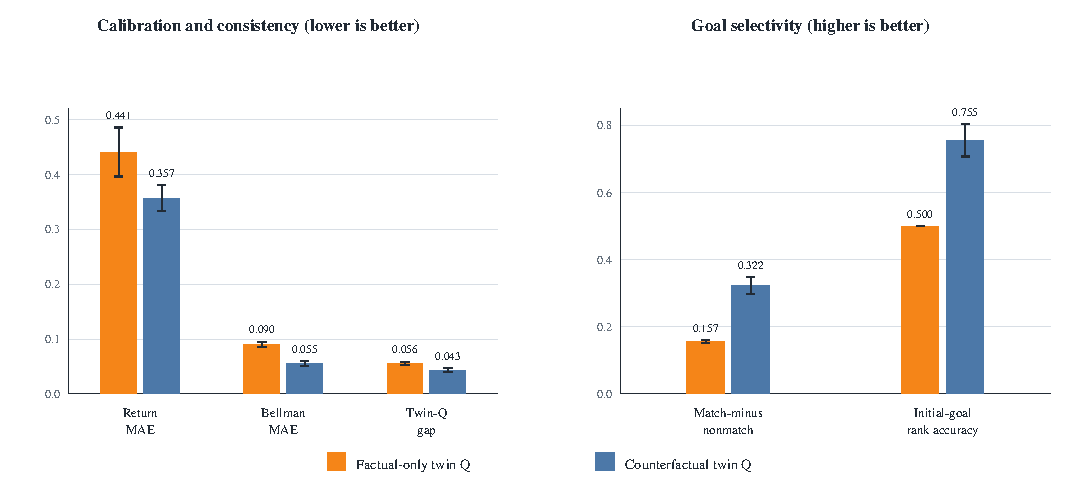
\includegraphics[width=\textwidth]{figures/figure_14.pdf}
\caption*{\textbf{Figure 14.} Held-out Study IV metrics after 10,000 updates. Bars are means over three Q initializations and whiskers are population standard deviations. Return MAE uses factual recorded behavior-policy returns; Bellman MAE evaluates one-step self-consistency for both goal queries under the frozen actor. Goal-rank accuracy is measured on successful initial states.}
\end{figure}
\begin{table}[H]
\centering
\begingroup
\footnotesize
\setlength{\tabcolsep}{3.5pt}
\renewcommand{\arraystretch}{1.15}
\begin{tabularx}{\textwidth}{@{} >{\hsize=1.318\hsize\RaggedRight\arraybackslash}X >{\hsize=0.865\hsize\RaggedRight\arraybackslash}X >{\hsize=0.881\hsize\RaggedRight\arraybackslash}X >{\hsize=0.936\hsize\RaggedRight\arraybackslash}X @{}}
\rowcolor{brandblue}
\color{white}\textbf{Held-out metric} & \color{white}\textbf{Factual-only} & \color{white}\textbf{Counterfactual} & \color{white}\textbf{Counterfactual change} \\
Factual return MAE (lower) & 0.441 +/- 0.045 & 0.357 +/- 0.024 & -0.084 (-19.0\%) \\
\rowcolor{rowgray}
Factual return bias (toward zero) & -0.178 +/- 0.064 & -0.165 +/- 0.043 & +0.014 \\
All-query Bellman MAE (lower) & 0.090 +/- 0.005 & 0.055 +/- 0.004 & -0.035 (-39.0\%) \\
\rowcolor{rowgray}
Twin-Q disagreement (lower) & 0.056 +/- 0.003 & 0.043 +/- 0.003 & -0.013 (-22.7\%) \\
Matching-minus-nonmatching value & 0.157 +/- 0.004 & 0.322 +/- 0.025 & +0.166 (+105.9\%) \\
\rowcolor{rowgray}
Successful initial goal rank & 0.500 +/- 0.000 & 0.755 +/- 0.048 & +25.5 pp \\
Mean nonmatching value & -0.202 +/- 0.064 & -0.354 +/- 0.030 & -0.152 (descriptive) \\
\bottomrule
\end{tabularx}
\endgroup
\caption*{\textbf{Table 15.} Final held-out means +/- population SD across three Q initializations. Lower nonmatching value is evidence of separation, not counterfactual calibration, because no unseen-goal return label exists.}
\end{table}
The counterfactual arm improves every primary qualification statistic. Factual return MAE falls by 19.0\% rather than trading factual calibration for goal separation. All-query Bellman error falls by 39.0\%, twin disagreement falls by 22.7\%, and the matching-minus-nonmatching gap more than doubles. Successful initial-state goal ranking moves from exactly chance in every factual-only seed to 68.75-79.69\% in the counterfactual seeds. Neither arm reproduces the original all-goals-high failure: the rate is 0.10\% for factual-only and zero for counterfactual.

\begin{table}[H]
\centering
\begingroup
\footnotesize
\setlength{\tabcolsep}{3.5pt}
\renewcommand{\arraystretch}{1.15}
\begin{tabularx}{\textwidth}{@{} >{\hsize=1.296\hsize\RaggedRight\arraybackslash}X >{\hsize=1.023\hsize\RaggedRight\arraybackslash}X >{\hsize=0.965\hsize\RaggedRight\arraybackslash}X >{\hsize=1.043\hsize\RaggedRight\arraybackslash}X >{\hsize=0.673\hsize\RaggedRight\arraybackslash}X @{}}
\rowcolor{brandblue}
\color{white}\textbf{Next positive reward} & \color{white}\textbf{Held-out transitions} & \color{white}\textbf{Factual-only MAE} & \color{white}\textbf{Counterfactual MAE} & \color{white}\textbf{Difference} \\
1 action & 64 & 0.834 & 0.764 & -0.070 \\
\rowcolor{rowgray}
2-5 actions & 245 & 0.857 & 0.800 & -0.058 \\
6-15 actions & 493 & 0.877 & 0.822 & -0.055 \\
\rowcolor{rowgray}
16+ actions & 654 & 0.491 & 0.452 & -0.039 \\
No future reward & 4,641 & 0.360 & 0.265 & -0.095 \\
\bottomrule
\end{tabularx}
\endgroup
\caption*{\textbf{Table 16.} Factual return MAE by distance from the next positive recorded reward. Counterfactual training improves every bin, including the 654 transitions more than the Dreamer imagination horizon of 15 actions from reward.}
\end{table}
\reportsubsection{10.4 Interpretation and claim boundary}
\begin{center}
\fcolorbox{brandblue}{calloutblue}{%
\begin{minipage}{0.94\linewidth}
\textbf{Qualification result.} Ordinary one-step counterfactual twin-Q training creates substantially stronger two-goal separation while also improving factual calibration, Bellman consistency, and twin agreement. It does so without an oracle value or the original critic bootstrap. This is sufficient to advance the mechanism into a normal CRL-pipeline test, but not sufficient to call the critic a validated actor or rehearsal teacher.
\end{minipage}}
\end{center}
The original theory was incorrect in its simple form. Weak reward/continuation conditioning did not merely propagate into an otherwise sound critic: repairing those heads left the existing critic flat, whereas directly changing the new critic's labelled TD objective produced selectivity. The remaining problem is critic training and target construction itself. The result also shows why a no-bootstrap critic target is unnecessary: one-step TD backs up sparse rewards repeatedly through recorded replay, including trajectories whose reward lies beyond the 15-step imagination horizon.

The positive result remains deliberately narrow. The three repetitions are Q initialization seeds on one fixed Dreamer checkpoint and one replay split. Held-out factual targets are behavior-policy returns rather than exact returns under the frozen actor, and no counterfactual ground-truth return exists. The actor is frozen, the new critics are not installed into Dreamer, no policy improvement or imagined rehearsal is attempted, and only GoToDoor and Fetch are queried. Absolute factual errors remain material, especially within 15 actions of sparse reward. The next study must test the same target online in the ordinary CRL pipeline before it is allowed to teach an actor.

\reportsection{11. Implications for continual imagined rehearsal}
\reportsubsection{11.1 What the combined evidence establishes}
\begin{itemize}
\item \textbf{Catastrophic forgetting is measurable in MiniGrid.} GoToDoor supplies a strong, replicated acquisition-to-collapse signal, so Dreamer is not too strong for the selected sequential regime.
\item \textbf{Memory availability is not enough.} Both reservoir arms retain old goal episodes, yet old behavior degrades and late tasks become harder to acquire.
\item \textbf{Uniform replay is a scientifically useful but poor performance baseline.} Its low current-task share reveals why CIR was intended to keep the actor focused on the current posterior while components rehearse old goals.
\item \textbf{Reward and continuation semantics are directly repairable.} Counterfactual labels create the intended same-state separation without changing the representation or behavior objectives.
\item \textbf{The original critic failure is not simple upstream propagation.} It remains optimistic and goal-insensitive after reward and continuation repair, so weak head conditioning was not the sole cause.
\item \textbf{Ordinary counterfactual TD is a promising critic mechanism.} A separate EMA twin-Q learner improves factual calibration and doubles same-state goal separation without an oracle value or the original critic bootstrap.
\item \textbf{Factual acquisition survives the semantic intervention.} The pilot outperforms its matched reference in both policy modes, but one training seed cannot establish a general behavioral advantage.
\item \textbf{Forward transfer is not yet present.} The next intervention should first solve acquisition and retention; positive transfer remains a later criterion.
\end{itemize}
\reportsubsection{11.2 Recommended next experimental sequence}
The next run should not add a gate around the current teacher. Gating decides \emph{when} to use a signal; it does not make an overoptimistic or goal-insensitive critic correct. Study IV has now supplied a qualified target construction, so the evidence supports the following staged mechanistic programme:

\begin{enumerate}
\item Treat counterfactual reward and continuation training as a validated head-level intervention, while retaining the ordinary factual losses and stopped feature path used in the pilot.
\item Install the Study IV one-step EMA twin-Q target into the ordinary two-goal CRL training pipeline while initially keeping its output out of the actor loss. Preserve the dose-matched factual twin-Q arm and the existing Dreamer critic as controls.
\item Repeat held-out factual calibration, same-state goal ranking, Bellman residual, twin disagreement, distance-to-reward, and source-parameter integrity checks during online training. Add fresh-policy factual returns so behavior-policy mismatch can be quantified.
\item Only after the online critic remains stable should the actor receive its target. Compare critic-guided learning against a frozen-actor control and reward-only actor training before allowing the critic into imagined rehearsal.
\item Retain both reservoir allocations. Uniform replay remains the primary component-preservation baseline; 50:50 remains the ordinary-replay comparator that CIR must beat on current acquisition.
\item Only after the repaired teacher passes online real-state and imagined-path audits should a safety gate be calibrated. The gate should veto uncertain or out-of-distribution rehearsal, not compensate for known target bias.
\item Repeat the four-task stream over more seeds after the intervention is fixed, then carry the validated mechanism through Fetch-style simulated manipulation, redesigned RLScape, and finally the CoBot320Pi arm.
\end{enumerate}
\begin{center}
\fcolorbox{brandblue}{calloutblue}{%
\begin{minipage}{0.94\linewidth}
\textbf{Immediate decision.} The head intervention and the offline counterfactual twin-Q target have passed their respective qualification gates. The next experiment should move the same twin-Q target into the usual two-goal CRL pipeline, without yet granting it control of the actor.
\end{minipage}}
\end{center}
\reportsubsection{11.3 Relationship to the RLScape evidence}
The MiniGrid baseline does not replace RLScape; it removes one major ambiguity from it. RLScape's large click action space and Berry Bones task could have masqueraded as agent failure. MiniGrid uses seven shared actions and still reproduces the two most important mechanistic findings: weak counterfactual reward semantics and severe critic optimism. The critic problem is therefore unlikely to be only an RLScape action-resolution artifact. MiniGrid now also supplies a cheap candidate solution: event-local counterfactual labels plus conservative one-step twin-Q bootstrapping. It should be validated in MiniGrid's online pipeline before translation to RLScape's larger action space.

\reportsection{12. Limitations and claim boundaries}
\begin{enumerate}
\item \textbf{Three baseline seeds and one pilot seed.} Study II repetition is sufficient to reveal qualitative failure but not small arm differences; Study III establishes a causal component result in one matched case, not population-level behavioral efficacy.
\item \textbf{Three Q seeds are not three environment seeds.} Study IV repeats critic initialization on one frozen Dreamer checkpoint, replay selection, and held-out bank. Its low variance does not measure training-data or representation uncertainty.
\item \textbf{Fifty episodes per policy mode and checkpoint.} Paired resets control comparisons; each individual proportion retains binomial uncertainty.
\item \textbf{Task difficulty remains unequal.} GoToObject is weak across arms, and PutNear is strongly sensitive to current-task exposure. Aggregate forgetting cannot replace task-level reporting.
\item \textbf{No return-to-A phase.} The study measures retention at later checkpoints, not rapid reacquisition. The immutable 800k checkpoints allow a later continuation.
\item \textbf{No imagined-rehearsal intervention.} Studies III and IV change head or offline critic training, not actor adaptation. They do not show that reward-only, counterfactual, critic-guided, or gated rehearsal succeeds in MiniGrid.
\item \textbf{No forgetting test in the pilot.} Study III contains only GoToDoor Phase A. Its zero numerical forgetting is structural and must not be interpreted as retention.
\item \textbf{Independent diagnostic banks across runs.} Standard and pilot head audits each hold states fixed across goal queries, but use their own final replay banks. Cross-run prediction magnitudes are descriptive; the within-run factual-versus-wrong-goal contrasts carry the causal semantic claim.
\item \textbf{No online twin-Q test.} Study IV freezes the representation and actor, trains from a fixed replay bank, and never installs the new Q systems into Dreamer. It cannot measure representation drift, feedback with data collection, or policy improvement.
\item \textbf{Counterfactual outcomes lack oracle returns.} Goal-query differences and event-local Bellman targets are valid diagnostics, but only factual recorded trajectories receive realized behavior-return calibration labels.
\item \textbf{Fixed banks condition every diagnostic.} Study II and III audits use final uniform-replay banks; Study IV uses one fixed 50:50-replay split. Identical within-study evidence improves arm comparability but limits distributional coverage.
\item \textbf{One reduced Dreamer configuration.} Results are conditional on the 12M preset, train ratio 32, 100-action horizon, fixed missions, and four-task order.
\item \textbf{One serial hardware run.} Runtime demonstrates feasibility on the RTX 4090, not cross-platform performance.
\end{enumerate}
\reportsection{13. Conclusion}
Together, the four MiniGrid studies establish a fast and revealing mechanism-development tier for CIR. The independent audition rejected an overconfident task-matching assumption. The sequential baseline then completed 7.2 million training steps, 75,600 paired evaluation episodes, and 90 read-only component audits in 30.17 hours without a failed scientific unit. Dreamer is not too strong for this regime: catastrophic forgetting is large, late-task acquisition is replay-sensitive, and forward transfer is absent.

The baseline outcome is mechanistic. Uniform reservoir replay preserves data but starves current learning; 50:50 replay improves acquisition but does not preserve competence. Reward heads recognize factual events without reliably encoding which goal those events satisfy. Critics become grossly optimistic on real states, slow critics repeat the bias, and actor-selected imagination amplifies bootstrap-dominated targets.

The counterfactual-head pilot turns one diagnosis into a causal result. Explicit wrong-goal labels reduce nonmatching completion reward to approximately two parts per million and correctly mark the same physical event as continuing for other goals, while factual GoToDoor acquisition remains strong. Yet the unchanged critic values all six goal queries almost equally, and its wrong-goal imagined targets remain 98.96-100\% bootstrap across the tested horizons. Reward and continuation semantics can therefore be repaired independently, but the critic does not become a safe teacher merely because its upstream heads are correct.

The twin-Q qualification supplies the next causal step. Direct counterfactual critic labels improve factual calibration by 19\%, reduce all-query Bellman error by 39\%, double the matching-versus-nonmatching value gap, and raise successful initial-state goal ranking from chance to 75.5\%. The new critics remain conservative and are not yet validated teachers, but they avoid both an oracle return and the known-bad original value bootstrap. The simple theory that weak heads merely propagated optimism into the critic is therefore rejected; critic objective and target construction are independent mechanisms.

The next decision is now concrete: move the qualified one-step counterfactual EMA twin-Q target into the usual two-goal CRL pipeline, retain the factual-only twin-Q and original critic controls, and keep the actor isolated until real-state calibration remains stable online. Reward-only imagined rehearsal remains the approved actor reference, standard critic-bootstrapped IR remains a negative control, and gating remains premature until the teaching signal passes both online and imagined-path audits.

\clearpage
\reportsection{Appendix A. Seed-level final results}
\begin{table}[H]
\centering
\begingroup
\scriptsize
\setlength{\tabcolsep}{3.5pt}
\renewcommand{\arraystretch}{1.15}
\begin{tabularx}{\textwidth}{@{} >{\hsize=1.071\hsize\RaggedRight\arraybackslash}X >{\hsize=0.988\hsize\RaggedRight\arraybackslash}X >{\hsize=0.988\hsize\RaggedRight\arraybackslash}X >{\hsize=0.988\hsize\RaggedRight\arraybackslash}X >{\hsize=0.988\hsize\RaggedRight\arraybackslash}X >{\hsize=0.988\hsize\RaggedRight\arraybackslash}X >{\hsize=0.988\hsize\RaggedRight\arraybackslash}X @{}}
\rowcolor{brandblue}
\color{white}\textbf{Task} & \color{white}\textbf{Seed 0 Samp.} & \color{white}\textbf{Seed 0 Det.} & \color{white}\textbf{Seed 1 Samp.} & \color{white}\textbf{Seed 1 Det.} & \color{white}\textbf{Seed 2 Samp.} & \color{white}\textbf{Seed 2 Det.} \\
GoToDoor & 92\% & 90\% & 0\% & 0\% & 46\% & 48\% \\
\rowcolor{rowgray}
Fetch & 4\% & 2\% & 60\% & 56\% & 4\% & 6\% \\
GoToObject & 0\% & 0\% & 70\% & 56\% & 40\% & 42\% \\
\rowcolor{rowgray}
PutNear & 92\% & 90\% & 100\% & 100\% & 62\% & 74\% \\
UnlockPickup & 0\% & 0\% & 0\% & 0\% & 0\% & 0\% \\
\rowcolor{rowgray}
PickupDist & 4\% & 4\% & 0\% & 0\% & 0\% & 2\% \\
\bottomrule
\end{tabularx}
\endgroup
\caption*{\textbf{Table A1.} Final sampled and deterministic success for every run. Each cell contains 50 episodes.}
\end{table}
\reportsection{Appendix B. Checkpoint means}
\begin{table}[H]
\centering
\begingroup
\scriptsize
\setlength{\tabcolsep}{3.5pt}
\renewcommand{\arraystretch}{1.15}
\begin{tabularx}{\textwidth}{@{} >{\hsize=1.376\hsize\RaggedRight\arraybackslash}X >{\hsize=0.953\hsize\RaggedRight\arraybackslash}X >{\hsize=0.953\hsize\RaggedRight\arraybackslash}X >{\hsize=0.953\hsize\RaggedRight\arraybackslash}X >{\hsize=0.953\hsize\RaggedRight\arraybackslash}X >{\hsize=0.953\hsize\RaggedRight\arraybackslash}X >{\hsize=0.953\hsize\RaggedRight\arraybackslash}X >{\hsize=0.953\hsize\RaggedRight\arraybackslash}X >{\hsize=0.953\hsize\RaggedRight\arraybackslash}X @{}}
\rowcolor{brandblue}
\color{white}\textbf{Task} & \color{white}\textbf{25k S} & \color{white}\textbf{25k D} & \color{white}\textbf{50k S} & \color{white}\textbf{50k D} & \color{white}\textbf{75k S} & \color{white}\textbf{75k D} & \color{white}\textbf{100k S} & \color{white}\textbf{100k D} \\
GoToDoor & 0.0\% & 0.0\% & 0.0\% & 0.0\% & 31.3\% & 28.7\% & 46.0\% & 46.0\% \\
\rowcolor{rowgray}
Fetch & 0.0\% & 0.0\% & 0.7\% & 0.7\% & 8.7\% & 8.7\% & 22.7\% & 21.3\% \\
GoToObject & 0.0\% & 0.0\% & 4.7\% & 5.3\% & 14.7\% & 14.7\% & 36.7\% & 32.7\% \\
\rowcolor{rowgray}
PutNear & 2.0\% & 0.0\% & 20.0\% & 15.3\% & 0.0\% & 0.0\% & 84.7\% & 88.0\% \\
UnlockPickup & 0.0\% & 0.0\% & 0.0\% & 0.0\% & 0.0\% & 0.0\% & 0.0\% & 0.0\% \\
\rowcolor{rowgray}
PickupDist & 0.0\% & 0.0\% & 0.7\% & 0.0\% & 3.3\% & 4.0\% & 1.3\% & 2.0\% \\
\bottomrule
\end{tabularx}
\endgroup
\caption*{\textbf{Table B1.} Mean success across three seeds. S = sampled; D = deterministic.}
\end{table}
\reportsection{Appendix C. Reproducibility package}
The report directory contains compact evidence packages for all four studies: immutable specifications, complete aggregate evaluation tables, supervisor provenance, replay-allocation summaries, and every per-checkpoint head and critic summary used here, plus the complete Study IV final-run table. Raw replay archives, checkpoints, JSONL logs, prediction tensors, latent caches, and rollout shards remain authoritative on the RTX 4090 under /home/localadmin/experiment\_logs/minigrid/.

\begin{table}[H]
\centering
\begingroup
\footnotesize
\setlength{\tabcolsep}{3.5pt}
\renewcommand{\arraystretch}{1.15}
\begin{tabularx}{\textwidth}{@{} >{\hsize=0.643\hsize\RaggedRight\arraybackslash}X >{\hsize=1.357\hsize\RaggedRight\arraybackslash}X @{}}
\rowcolor{brandblue}
\color{white}\textbf{Artifact} & \color{white}\textbf{Role} \\
\path{data/experiment_spec.json} & Pinned task, model, evaluation, pairing, and dependency specification \\
\rowcolor{rowgray}
\path{data/evaluation_summary.csv} & All 144 checkpoint-policy conditions \\
\path{data/run_summary.csv} & Per-task and per-seed training/final metrics \\
\rowcolor{rowgray}
\path{data/task_summary.csv} & Cross-seed task aggregation \\
\path{data/pairwise_difficulty.csv} & Predeclared pairwise decisions \\
\rowcolor{rowgray}
\path{data/supervisor_status.json} & Commands, timestamps, attempts, return codes, and runtime versions \\
\path{data/sequential_baseline/analysis/} & All Study II behavior, replay, drift, and component aggregate tables \\
\rowcolor{rowgray}
\path{data/sequential_baseline/diagnostics/} & Compact summaries and specifications for all 90 read-only audits \\
\path{data/sequential_baseline/supervisor_status.json} & Complete Study II commands, attempts, timings, and terminal state \\
\rowcolor{rowgray}
\path{data/counterfactual_heads_phase_a_pilot/} & Study III specification, pairing, analysis, diagnostic summaries, and source hashes \\
\path{data/twin_q_qualification/} & Study IV specification, final per-seed/aggregate metrics, integrity hashes, and provenance \\
\rowcolor{rowgray}
\path{build_report.py} & Reproducible vector-PDF builder \\
\bottomrule
\end{tabularx}
\endgroup
\caption*{\textbf{Table C1.} Portable report package. Raw run artifacts remain authoritative.}
\end{table}
Regenerate with:
\begin{quote}\small\ttfamily
/home/zythax/.cache/codex-runtimes/codex-primary-runtime/dependencies/python/bin/python3.12\newline
reports/minigrid\_baseline\_report/build\_report.py
\end{quote}

\clearpage
\reportsection{Appendix D. Study II task-level outcomes}
\begin{table}[H]
\centering
\begingroup
\scriptsize
\setlength{\tabcolsep}{3.5pt}
\renewcommand{\arraystretch}{1.15}
\begin{tabularx}{\textwidth}{@{} >{\hsize=0.850\hsize\RaggedRight\arraybackslash}X >{\hsize=1.071\hsize\RaggedRight\arraybackslash}X >{\hsize=1.055\hsize\RaggedRight\arraybackslash}X >{\hsize=1.024\hsize\RaggedRight\arraybackslash}X >{\hsize=1.039\hsize\RaggedRight\arraybackslash}X >{\hsize=0.976\hsize\RaggedRight\arraybackslash}X >{\hsize=0.929\hsize\RaggedRight\arraybackslash}X >{\hsize=1.055\hsize\RaggedRight\arraybackslash}X @{}}
\rowcolor{brandblue}
\color{white}\textbf{Arm} & \color{white}\textbf{Task} & \color{white}\textbf{Sampled acq.} & \color{white}\textbf{Sampled final} & \color{white}\textbf{Sampled BWT} & \color{white}\textbf{Det. acq.} & \color{white}\textbf{Det. final} & \color{white}\textbf{Det. BWT} \\
FIFO & GoToDoor & 95.3\% & 0.7\% & -94.7 pp & 95.3\% & 0.0\% & -95.3 pp \\
\rowcolor{rowgray}
FIFO & Fetch & 18.7\% & 0.0\% & -18.7 pp & 12.0\% & 0.0\% & -12.0 pp \\
FIFO & GoToObject & 0.0\% & 2.0\% & +2.0 pp & 0.0\% & 4.7\% & +4.7 pp \\
\rowcolor{rowgray}
FIFO & PutNear & 67.3\% & 67.3\% & +0.0 pp & 66.7\% & 66.7\% & +0.0 pp \\
Uniform & GoToDoor & 78.0\% & 0.0\% & -78.0 pp & 74.0\% & 0.0\% & -74.0 pp \\
\rowcolor{rowgray}
Uniform & Fetch & 1.3\% & 0.0\% & -1.3 pp & 0.0\% & 0.0\% & +0.0 pp \\
Uniform & GoToObject & 0.0\% & 0.0\% & +0.0 pp & 0.0\% & 0.0\% & +0.0 pp \\
\rowcolor{rowgray}
Uniform & PutNear & 0.0\% & 0.0\% & +0.0 pp & 0.0\% & 0.0\% & +0.0 pp \\
50:50 & GoToDoor & 92.0\% & 28.7\% & -63.3 pp & 94.7\% & 28.7\% & -66.0 pp \\
\rowcolor{rowgray}
50:50 & Fetch & 55.3\% & 0.0\% & -55.3 pp & 58.7\% & 0.0\% & -58.7 pp \\
50:50 & GoToObject & 30.0\% & 0.0\% & -30.0 pp & 28.0\% & 0.0\% & -28.0 pp \\
\rowcolor{rowgray}
50:50 & PutNear & 0.0\% & 0.0\% & +0.0 pp & 0.0\% & 0.0\% & +0.0 pp \\
\bottomrule
\end{tabularx}
\endgroup
\caption*{\textbf{Table D1.} Mean immediate post-acquisition success, final success, and backward transfer over three seeds. BWT = final minus post-acquisition.}
\end{table}
The underlying transfer\_and\_forgetting.csv retains all 72 task-seed-mode rows, including initial, pretraining, peak post-acquisition, final, forward-transfer, and forgetting values. The report uses means only for legibility; seed-level results remain available for uncertainty analysis and later paired intervention comparisons.

\reportsection{Appendix E. Study II audit inventory and integrity}
\begin{table}[H]
\centering
\begingroup
\footnotesize
\setlength{\tabcolsep}{3.5pt}
\renewcommand{\arraystretch}{1.15}
\begin{tabularx}{\textwidth}{@{} >{\hsize=0.602\hsize\RaggedRight\arraybackslash}X >{\hsize=0.865\hsize\RaggedRight\arraybackslash}X >{\hsize=1.532\hsize\RaggedRight\arraybackslash}X @{}}
\rowcolor{brandblue}
\color{white}\textbf{Evidence} & \color{white}\textbf{Scope} & \color{white}\textbf{Integrity / role} \\
Evaluation matrix & 1,512 conditions; 75,600 episodes & Exact episode/reset counts; paired modes; unchanged checkpoint digests \\
\rowcolor{rowgray}
Replay allocation & 288 logged snapshots & Observed goal fractions and reservoir occupancy \\
Goal-specific losses & 288 logged snapshots & Reward, continuation, value, policy, representation, and dynamics loss by replay goal \\
\rowcolor{rowgray}
Head audits & 45 jobs; five boundaries x nine runs & Identical state bank per seed; all six goal queries; unchanged parameters \\
Critic provenance & 45 jobs; H=1/3/6/15 & 32 posterior samples; actor and recorded actions; unchanged parameters \\
\rowcolor{rowgray}
Actor drift & 144 adjacent-boundary comparisons & Same states and factual goal query before/after each phase \\
\bottomrule
\end{tabularx}
\endgroup
\caption*{\textbf{Table E1.} Study II visibility and integrity evidence.}
\end{table}
The compact report package is approximately 20 MB. The excluded raw remote evidence includes about 700 MB of diagnostic predictions and per-episode critic shards plus the full 80 GB experiment tree. Compact summaries record source selections, specification digests, row counts, and before/after parameter hashes so every reported aggregate can be traced back to its immutable job.

\clearpage
\reportsection{Appendix F. Study III evidence and provenance}
\begin{table}[H]
\centering
\begingroup
\footnotesize
\setlength{\tabcolsep}{3.5pt}
\renewcommand{\arraystretch}{1.15}
\begin{tabularx}{\textwidth}{@{} >{\hsize=0.591\hsize\RaggedRight\arraybackslash}X >{\hsize=0.936\hsize\RaggedRight\arraybackslash}X >{\hsize=1.474\hsize\RaggedRight\arraybackslash}X @{}}
\rowcolor{brandblue}
\color{white}\textbf{Evidence} & \color{white}\textbf{Scope} & \color{white}\textbf{Integrity / role} \\
Training & 1 task; seed 0; 200,000 steps & One completed attempt; 9 immutable snapshots; exact 200k milestone \\
\rowcolor{rowgray}
Evaluation & 18 conditions; 900 episodes & 50 episodes and resets per mode-checkpoint; paired RNG; unchanged checkpoints \\
Head audits & 0 and 200k; 972 states at 200k & 32 fixed episodes; six goal queries; unchanged parameters \\
\rowcolor{rowgray}
Critic provenance & 0 and 200k; H=1/3/6/15 & 32 posterior samples; actor/recorded controls; reward/bootstrap decomposition \\
Portable evidence & Spec, status, pairing, analysis, banks, summaries & Principal SHA-256 hashes recorded in PROVENANCE.md \\
\rowcolor{rowgray}
Raw source & \path{counterfactual_heads_phase_a_pilot_v1} & Immutable office-4090 root; checkpoints and replay excluded \\
\bottomrule
\end{tabularx}
\endgroup
\caption*{\textbf{Table F1.} Study III completion and provenance inventory. The diagnostic bank-selection job is infrastructure and is not counted among the four read-only head/critic jobs.}
\end{table}
The experiment is pinned to Git commit f5e6e256bed9d4e7cec59108a3f8405033ab71f1 and specification digest 7a8fd6d11a1823720a0982179602ca2e0e813aea659e7516be440ab7f80257a9. The authoritative raw root is /home/localadmin/experiment\_logs/minigrid/counterfactual\_heads\_phase\_a\_pilot\_v1. The portable PROVENANCE.md records the remote root, copied artifact scope, and principal source hashes. All copied principal files were verified byte-for-byte after transfer.

\clearpage
\reportsection{Appendix G. Study IV evidence and provenance}
\begin{table}[H]
\centering
\begingroup
\footnotesize
\setlength{\tabcolsep}{3.5pt}
\renewcommand{\arraystretch}{1.15}
\begin{tabularx}{\textwidth}{@{} >{\hsize=0.602\hsize\RaggedRight\arraybackslash}X >{\hsize=0.959\hsize\RaggedRight\arraybackslash}X >{\hsize=1.439\hsize\RaggedRight\arraybackslash}X @{}}
\rowcolor{brandblue}
\color{white}\textbf{Evidence} & \color{white}\textbf{Scope} & \color{white}\textbf{Integrity / role} \\
Source & 50:50 seed 0 at 400k & Immutable checkpoint and exact 400k replay milestone \\
\rowcolor{rowgray}
Latent banks & 384 episodes; 18,723 states & Episode-disjoint train/held-out split; balanced goal/outcome strata \\
Transitions & 12,242 train; 6,097 held-out & Recorded one-step posterior transitions; seven discrete actions \\
\rowcolor{rowgray}
Twin-Q training & 2 arms x 3 Q seeds x 10,000 updates & Six complete resumable runs; final and aggregate tables \\
Dreamer integrity & 506 arrays; all namespaces & Before/after SHA-256 groups identical \\
\rowcolor{rowgray}
Portable evidence & 7 copied CSV/JSON sources plus provenance & Local/remote SHA-256 hashes match byte-for-byte \\
Raw source & \path{twin_q_qualification_400k_v2} & Latent caches and 23 MB Q checkpoints retained on office-4090 \\
\bottomrule
\end{tabularx}
\endgroup
\caption*{\textbf{Table G1.} Study IV completion and provenance inventory.}
\end{table}
The final experiment is pinned to Git commit e1d5d2a37ea9119a30475dd473c2244283775be2. The authoritative raw root is /home/localadmin/experiment\_logs/minigrid/twin\_q\_qualification\_400k\_v2. The portable PROVENANCE.md records the exact copied-file SHA-256 hashes, remote root, bank sizes, and timestamps. All seven principal files were verified byte-for-byte after transfer. The source checkpoint's 506-array digest is 16a742de354ed5b1fe9e0f9ea400e952ed80dcf45d3aed4c19f0c09c6a01e46f both before and after latent encoding.

\reportsection{References}
\hangindent=1.2em\hangafter=1 [1] Kirkpatrick, J. et al. (2017). Overcoming catastrophic forgetting in neural networks. \emph{Proceedings of the National Academy of Sciences}, 114(13), 3521-3526.\par
\hangindent=1.2em\hangafter=1 [2] Chevalier-Boisvert, M. et al. (2023). MiniGrid and MiniWorld: Modular and customizable reinforcement learning environments for goal-oriented tasks. \emph{Advances in Neural Information Processing Systems}, 36.\par
\hangindent=1.2em\hangafter=1 [3] Hafner, D., Pasukonis, J., Ba, J., and Lillicrap, T. (2023). Mastering diverse domains through world models. \emph{arXiv:2301.04104}.\par
\end{document}
